%%%%%%%%%%%%%%%%%%%%%%%%%%%%%%%%%%%%%%%%%%%%%%%%%%%%%%%%%%%%%%%%%%%%%%%%%
%%   CHAPTER: EARLY LIFE
%%%%%%%%%%%%%%%%%%%%%%%%%%%%%%%%%%%%%%%%%%%%%%%%%%%%%%%%%%%%%%%%%%%%%%%%%

\renewcommand{\chapterfolder}{early_life/}
\chapterimage{cover/early_life} % Chapter heading image
\chapter{Early Life}


\vspace*{-0.4in}
\epigraph{I used to feel guilty in Cambridge that I spent all day playing games, while I was supposed to be doing mathematics. \\ Then . . . I realized that playing games \emph{is} math.}{John H. Conway}
\vspace*{0.4in}


\noindent Conway's Game of Life\footnote{Named for its inventor, John H. Conway.} is a process that takes place on an infinite square grid, where each square can be in one of two states: \textbf{alive} or \textbf{dead}\index{alive}\index{dead} (depicted via black and white squares, respectively, in this book). The squares (which we typically call \textbf{cells})\index{cell} then evolve in discrete timesteps (called \textbf{generations} or\index{cellular automaton} \textbf{ticks})\index{generation}\index{tick} according to the following two rules:\smallskip

\begin{itemize}
	\item If a cell is alive, it survives to the next generation if it has 2 or 3 live neighbors; otherwise it dies.\smallskip
	
	\item If a cell is dead, it comes to life in the next generation if it has exactly 3 live neighbors; otherwise it stays dead.\smallskip
\end{itemize}

We note that these rules are applied to every square in the grid simultaneously, and a ``neighbor'' in these rules refers to any of the 8 cells that it touches either along a side or at a corner, as in Figure~\ref{fig:neighborhood}. As an example of how these rules work, consider what happens to the straight line of 4 alive cells depicted in Figure~\ref{fig:first_example}. The leftmost and rightmost cells in the line both only have one live neighbor, so they die, while the two central cells above and below the line each have exactly 3 live neighbors, so they come to life. This leaves us with a $3 \times 2$ rectangle of live cells, so we say that the line of 4 live cells is a \textbf{parent}\index{parent} of the $3 \times 2$ rectangle of live cells, or equivalently that the $3 \times 2$ rectangle is a \textbf{child}\index{child} of the line of 4 cells. We then apply the evolution rules again: this time, the two central cells in the rectangle are overpopulated and die, while the dead cells to their immediate left and right have exactly 3 live neighbors and thus come to life.

\begin{figure}[!htb]
	\centering
	\begin{minipage}[b]{0.38\textwidth}
		\centering
		\patternimg{0.125}{neighborhood}
		\caption{A live cell (in black) in the middle and its 8 neighbors (in \bgbox{aquaback}{aqua}).}\label{fig:neighborhood}
	\end{minipage}\hfill
	\begin{minipage}[b]{0.58\textwidth}
		\centering
		\embedlink{first_example}{\vcenteredhbox{\patternimg{0.125}{first_example_0}} \vcenteredhbox{\genarrow{1}} \vcenteredhbox{\patternimg{0.125}{first_example_1}} \vcenteredhbox{\genarrow{1}} \vcenteredhbox{\patternimg{0.125}{first_example_2}}}
		\caption{A line of four alive cells takes two generations to evolve into a stable object called a \textbf{beehive}\index{beehive}. The $3 \times 2$ object in the middle is sometimes called a \textbf{pre-beehive}.}\label{fig:first_example}\index{pre-beehive}
	\end{minipage}
\end{figure}

After this point, if we apply the evolution rule again, nothing changes; each of the live cells have 2 live neighbors and thus live to the next generation, and no dead cell has 3 live neighbors, so they all stay dead. A pattern like this that remains unchanged from one generation to the next is called a \textbf{still life}.\index{still life}

As we saw in this example, there was no input on our part once the pattern started evolving: we just applied the game's rules and passively watched what happened from one generation to the next. Instead, the ``game'' in Life is the challenge of finding new and interesting patterns that evolve in unique and unexpected ways, and that is what this book is about. We will see patterns that move back and forth periodically between a finite number of different configurations, patterns that move through the Life grid over time, and patterns that create an infinitely growing family of other patterns. We will collide patterns with each other to create more complicated patterns, which we will then erase with even more patterns. We will construct logical circuitry with Life objects that allow us to simulate arbitrary computation within the Life universe, and we will construct patterns that do remarkable things like list the prime numbers or print out the decimal digits of $\pi$. And all of this will work simply based the two simple life and death rules we described earlier.

This all leads to a very natural question: why those rules? Why not have a dead cell come to life only in the case that it has exactly 4~live neighbors? Why not have a live cell stay alive if it has exactly 1, 2, 4, or 7 live neighbors? Indeed, there are $2^{18} = 262{\thousep}144$ distinct \textbf{Life-like cellular automata}:\index{Life-like} rules that can be applied to a 2D square grid of alive and dead cells that simply depend on the numbers of live and dead neighbors that lead to a cell staying alive or coming to life. However, the following three properties make Life special (but by no means unique):\smallskip

\begin{itemize}
	\item Its rules are \emph{simple}. For example, having a live cell stay alive if it has exactly 2 or 3 live neighbors is a more ``natural'' rule than having a live cell stay alive if it has exactly 1, 2, 4, or 7 live neighbors. This can be justified a bit by arguing that, to model something like a biological system, a cell should die of overcrowding if it has ``too many'' neighbors (e.g., since there won't be enough resources to support all of the live cells), and it should die of isolation if it has ``too few'' neighbors. The exact threshold for ``too many'' and ``too few'' is debatable, but pinned down at least somewhat by the next point.\smallskip
	
	\item It strikes a balance between being \emph{chaotic} and \emph{stable}. Many rules (e.g., almost any rule in which a cell is born when it has 2 live neighbors) cause far too many births for anything to stabilize. These rules are thus ``too chaotic'', making it almost impossible for us to construct interesting objects. On the other hand, most rules in which cells are \emph{not} born when they have $3$ (or fewer) live neighbors typically lead to patterns dying off extremely quickly and thus being ``too stable'' to be interesting. Life strikes a good balance of patterns typically staying alive but not overtaking the entire grid.\smallskip
	
	\item It is \emph{historical}. This is perhaps a bit of an unsatisfying reason, but part of the interest in Life simply comes from the fact that historically it is the most well-studied rule, and it is fun to see how far we can push one very well-studied rule, rather than dividing our attention and making moderate progress on multiple rules.\smallskip
\end{itemize}

Nonetheless, other birth and death rules are sometimes studied as well, and for brevity they are typically described using a \textbf{rulestring}\index{rulestring}\index{Bx/Sy|see {rulestring}} of the form \texttt{Bx/Sy}, where we replace ``\texttt{x}'' by all numbers of live neighbors that lead to the \textbf{b}irth of a dead cell, and we replace ``\texttt{y}'' by all numbers of live neighbors that lead to the \textbf{s}urvival of a live cell. For example, the Game of Life is described by the rulestring \texttt{B3/S23}. We will discuss other rules much later, in Chapter~\ref{chp:0e0p}, when we develop machinery that lets us run other cellular automata within Life.

There are also many more exotic ways to change the Game of Life beyond just changing the numbers of neighbors that cause cells to be alive. For example, we could have considered a \textbf{neighbor}\index{neighbor} of a cell to only be one of the 4 cells that shares one of its sides as in Figure~\ref{fig:vn_neighborhood}, not just a corner (this 4-cell neighborhood is called the \textbf{von Neumann neighborhood}\index{von Neumann neighborhood}, whereas the 8-cell neighborhood used by Life is called the \textbf{Moore neighborhood}\index{Moore neighborhood}). We could have considered a hexagonal or triangular grid instead of a square one, or a 1D or 3D grid instead of a 2D one. We could have constructed the game in such a way that not only the number of live neighbors matters, but also their relative positions---such rules are known as \textbf{isotropic rules}\index{isotropic}, or \textbf{INT rules}\index{INT rules} (short for ``isotropic non-totalistic'').

These are all potentially interesting modifications to make, and they fall under the general umbrella of \textbf{cellular automata}, but we will not consider them any further until Chapter~\ref{chp:0e0p}. Instead, as we emphasize one final time, our goal is to take the Game of Life cellular automaton itself and push it to its farthest limits.

\begin{figure}[!htb]
	\centering
	\patternimg{0.125}{vn_neighborhood}
	\caption{A live cell (in black) in the middle and the 4 cells in its von Neumann neighborhood (in \bgbox{aquaback}{aqua}).}\label{fig:vn_neighborhood}
\end{figure}


%%%%%%%%%%%%%%%%%%%%%%%%%%%%%%%%%%%%%%%%%%%%%%%%%%%%%%%%%%%%%%%%%%%%%%%%%
%%   SECTION: OUR FIRST TECHNIQUE: RANDOM FUMBLING
%%%%%%%%%%%%%%%%%%%%%%%%%%%%%%%%%%%%%%%%%%%%%%%%%%%%%%%%%%%%%%%%%%%%%%%%%
\section{Our First Technique: Random Fumbling}\label{sec:fumbling}

There are three main techniques used to construct objects in Life that behave in interesting and unusual ways:\smallskip

\begin{enumerate}
	\item[1)] We can write a computer program that searches for patterns with particular properties;\smallskip
	
	\item[2)] we can combine different already-known objects in such a way as to create new composite objects; or\smallskip
	
	\item[3)] we can put some random garbage on the Life board and evolve it, with the hope that something interesting pops out.\smallskip
\end{enumerate}

Option~(1) typically requires a fair bit of effort, as well as some knowledge of what exactly it is that we're searching for. Similarly, option~(2) is not yet possible for us since we are just starting out with Life and do not yet know of any objects that can be combined in an interesting way. We thus start with the extremely not clever option~(3): we try evolving a bunch of random patterns and see what is left of them after their chaos dies down.\footnote{This is not only \emph{our} approach to getting started with Life, but was also the historical approach: many of the patterns found in the first year or two of Life were found just by evolving many small configurations and looking at the results.} Our first example is presented in Figure~\ref{fig:random_1}, which is a random assortment of live cells that takes $116$~generations before stabilizing into several distinct objects. Random starting configurations like this one are sometimes called \textbf{soup}\index{soup}, and the objects that they leave behind are called \textbf{ash}\index{ash}.\footnote{The term ``ash'' refers to the fact that it is what is left after a pattern stops ``burning''.}

\begin{figure}[!htb]
	\centering\embedlink{random_1}{\vcenteredhbox{\patternimg{0.12}{random_1}} \vcenteredhbox{\genarrow{116}} \vcenteredhbox{\patternimg{0.085}{random_1_evolved}}}
	\caption{Evolving random junk is a decent way to find some small patterns to get us started in Life. The debris on the right introduces us to several still lifes, our first \textbf{oscillator}, and the \textbf{glider}.}\label{fig:random_1}
\end{figure}

In the ash, we see the beehive that we introduced earlier, as well as three other still lifes (i.e., patterns that do not change from one generation to the next). We also see an object called the \textbf{blinker}\index{blinker} that rotates itself by 90 degrees every generation. Patterns like this one, which cycle between finitely many different configurations, are called \textbf{oscillators}\index{oscillator}, and the configurations that they take on in individual generations are called \textbf{phases}\index{phase}. The most exotic object that we see in the ash is the one that is traveling by itself toward the top-right corner of the Life plane. An object that moves through the plane on its own is called a \textbf{spaceship}\index{spaceship}, and this particular one is called the \textbf{glider}\index{glider}.

Of course, there is nothing remotely special about the particular random configuration that we started with; we could generate other random starting configurations and see what types of ash pop out of them as well. In fact, Life is so chaotic and unpredictable that we could just change a single cell of the first configuration that we used, and we will likely get a completely different set of ash. Indeed, Figure~\ref{fig:random_2} demonstrates the drastic change that can often be made by altering just one cell in a pattern: by just changing one cell from alive to dead, we have made a new pattern that takes almost $3{\thousep}000$ generations to stabilize and results in ash that has over 20 times as many live cells. This new ash also has three additional still lifes in it that were not present in the previous ash. A summary of the ash objects we have seen so far is given in Figure~\ref{fig:first_objects}.

\begin{figure}[!ht]
	\centering\embedlink{random_2}{\vcenteredhbox{\centering\vcenteredhbox{\begin{tikzpicture}[scale=1.2, every node/.style={transform shape}]%
				\node[inner sep=0pt,anchor=south west] at (0,0) {\patternimg{0.1}{random_2}};
				\draw[white,line width=3pt,opacity=0.5](1.314,0.965) circle (0.165);
				\draw[redback2,line width=1pt](1.314,0.965) circle (0.165);
				\end{tikzpicture}}} \vcenteredhbox{\color{black}{$\xrightarrow{\text{\clock{0}{21} 2901}}$}} \vcenteredhbox{\gridbox{0.5pt}{\patternimg{0.08}{random_2_evolved}}}}
	\caption{Changing just a single cell (circled on the left in \bgbox{redback}{red}) from alive to dead in our random starting configuration causes its evolution to become completely different. It now takes over 25 times as long to stabilize and its ash contains three new types of still lifes (ponds, ships, and loaves).}\label{fig:random_2}
\end{figure}

Still lifes, oscillators, and spaceships are the three most basic types of objects that we will study in Life, and they form the building blocks of all of the more complicated patterns that we will construct. At this point though, there are some natural questions that we can ask about them. For example, we already saw the blinker, which oscillates back and forth between $2$ phases every $2$ generations. Do there exist oscillators that take longer to return to their original configuration? In other words, do there exist oscillators with \textbf{period}\index{period} larger than~$2$?

\begin{figure}[!htb]
	\centering\patternimglink{0.1}{first_objects}
	\caption{From left to right: seven still lifes, called the \textbf{block}, \textbf{tub}, \textbf{boat}, \textbf{ship}, \textbf{beehive}, \textbf{loaf} and \textbf{pond}, an oscillator called the \textbf{blinker}, and a spaceship called the \textbf{glider}. All of these objects frequently appear in the ash left behind by chaotic patterns.}\label{fig:first_objects}
\end{figure}

To answer this question, we simply continue not being clever: we evolve more and more random configurations of junk and record new objects that appear in the ash as we find them. Most of the new objects that we will find by doing this are additional still lifes, but new oscillators crop up from time to time as well. For example, the oscillator depicted in Figure~\ref{fig:pulsar}, which is called the \textbf{pulsar}\index{pulsar} and has period~$3$, appears rather frequently in random ash for its size.

\begin{figure}[!htb]
	\centering
	\embedlink{pulsar}{\vcenteredhbox{\patternimg{0.1}{pulsar_1}} \vcenteredhbox{\genarrow{1}} \vcenteredhbox{\patternimg{0.1}{pulsar_2}} \vcenteredhbox{\genarrow{1}} \vcenteredhbox{\patternimg{0.1}{pulsar_3}} \vcenteredhbox{\genarrow{1}} \vcenteredhbox{\patternimg{0.1}{pulsar_1}}}
	\caption{A period~3 oscillator called the \textbf{pulsar}.}\label{fig:pulsar}
\end{figure}

Some other oscillators that appear reasonably often in random ash are depicted in Figure~\ref{fig:random_oscillators}. Of particular note is the \textbf{pentadecathlon}\index{pentadecathlon}, which has a surprisingly large period of~15. This oscillator behaves somewhat differently than the other ones we have seen, as it pulsates and changes in size as it moves through its period---a property that will be very useful for us later on.

\begin{figure}[!htb]
	\centering\patternimglink{0.1}{random_oscillators}
	\caption{From left to right: three oscillators with period~2, called \textbf{toad}\index{toad}, \textbf{beacon}\index{beacon} and \textbf{clock}\index{clock}, and a period~15 oscillator called \textbf{pentadecathlon}.}\label{fig:random_oscillators}
\end{figure}

In the process of finding these oscillators, it is extremely likely that we will have also come across some other commonly occurring objects, such as the \textbf{lightweight spaceship}\index{lightweight!spaceship} (or \textbf{LWSS}\index{LWSS|see {lightweight spaceship}} for short) depicted in Figure~\ref{fig:lwss}. This is another spaceship, but this one moves orthogonally (i.e., directly north, south, east, or west), unlike the glider, which moves diagonally.

\begin{figure}[!htb]
	\centering\embedlink{lwss}{\vcenteredhbox{\patternimg{0.1}{lwss_1}} \vcenteredhbox{\genarrow{1}} \vcenteredhbox{\patternimg{0.1}{lwss_2}} \vcenteredhbox{\genarrow{1}} \vcenteredhbox{\patternimg{0.1}{lwss_3}} \vcenteredhbox{\genarrow{1}} \vcenteredhbox{\patternimg{0.1}{lwss_4}} \vcenteredhbox{\genarrow{1}} \vcenteredhbox{\patternimg{0.1}{lwss_5}}}
	\caption{The \textbf{lightweight spaceship}, which has period~4 and moves orthogonally to the right by $2$ cells every $4$ generations.}\label{fig:lwss}
\end{figure}

Slightly more rare than the lightweight spaceship are the \textbf{middleweight spaceship}\index{middleweight!spaceship} (or \textbf{MWSS}\index{MWSS|see {middleweight spaceship}}) and the \textbf{heavyweight spaceship}\index{heavyweight!spaceship} (or \textbf{HWSS}\index{HWSS|see {heavyweight spaceship}}),\footnote{In keeping with the ``\_\_\_\_weight spaceship'' naming convention, the glider was sometimes called the \textbf{featherweight spaceship}\index{featherweight spaceship|see {glider}} in the early days of Life, though this name is very rarely used now.} displayed in Figure~\ref{fig:lwss_mwss_hwss}. There are a handful of other objects that a lucky Life enthusiast might see while evolving random junk, but for the most part these are the ``standard'' naturally occurring objects. Some examples of random soups that generate more exotic objects are presented in Exercises~\ref{exer:natural_switch_engine} and~\ref{exer:random_symmetric}.

\begin{figure}[!htb]
	\centering\patternimglink{0.1}{lwss_mwss_hwss}
	\caption{From left to right: a lightweight, middleweight, and heavyweight spaceship. They all have period~$4$ and travel to the right $2$~cells every $4$~generations.}\label{fig:lwss_mwss_hwss}
\end{figure}


%%%%%%%%%%%%%%%%%%%%%%%%%%%%%%%%%%%%%%%%%%%%%%%%%%%%%%%%%%%%%%%%%%%%%%%%%
%%   SECTION: Common Evolutionary Sequences
%%%%%%%%%%%%%%%%%%%%%%%%%%%%%%%%%%%%%%%%%%%%%%%%%%%%%%%%%%%%%%%%%%%%%%%%%
\section{Common Evolutionary Sequences}\label{sec:evolution}\index{evolution}

We have seen plenty of interesting patterns so far simply by looking at the results of running random soups until they stabilize. However, we can also learn a lot by carefully watching the evolution of soups as they happen, as not only are there commonly occurring stable ash objects, but there are also commonly occurring unstable objects that explode and drive the evolution of those patterns. For example, one such object is the \textbf{T-tetromino}\index{T-tetromino},\footnote{A \textbf{polyomino}\index{polyomino} is a pattern made up of orthogonally connected live cells, and a \textbf{tetromino} is a polyomino with $4$ live cells. More generally, polyominoes with $2, 3, 4, \ldots, 8$ live cells are called \textbf{dominoes}, \textbf{triominoes}, \textbf{tetrominoes}, \textbf{pentominoes}, \textbf{hexominoes}, \textbf{heptominoes}, and \textbf{octominoes}.} which is a $4$-cell object that appears (for example) in generations $206$, $395$, and $568$ of the evolution of the soup from Figure~\ref{fig:random_2}. This tiny object (displayed in Figure~\ref{fig:t_tetromino}) explodes into an arrangement of $4$~blinkers that is called a \textbf{traffic light}.\index{traffic light} In fact, three traffic lights (and part of a fourth) can be seen in the ash of Figure~\ref{fig:random_2}, and the common T-tetromino explosion is exactly why blinkers appear in this formation so frequently.

\begin{figure}[!htb]
	\centering
	\embedlink{t_tetromino}{\vcenteredhboxfx{\patternimg{0.12}{t_tetromino_0}} \vcenteredhboxfx{\genarrow{1}} \vcenteredhboxfx{${}\!\!{}$\patternimg{0.12}{t_tetromino_1}} \vcenteredhboxfx{\genarrow{1}} \vcenteredhboxfx{\patternimg{0.1}{t_tetromino_2}} \vcenteredhboxfx{\genarrow{1}} \vcenteredhboxfx{${}\!\!\!\!{}$\patternimg{0.1}{t_tetromino_3}} \vcenteredhboxfx{\genarrow{1}} \vcenteredhboxfx{${}\!\!{}$\patternimg{0.1}{t_tetromino_4}} \vcenteredhboxfx{{} \ {}} \vcenteredhboxfx{{} \ {}}\\[0.1em]
		\vcenteredhboxfx{{\color{black}${} \ \ \ \ \cdots$}} \vcenteredhboxfx{\genarrow{1}} \vcenteredhboxfx{\patternimg{0.1}{t_tetromino_5}} \vcenteredhboxfx{\genarrow{1}} \vcenteredhboxfx{\patternimg{0.1}{t_tetromino_6}} \vcenteredhboxfx{\genarrow{1}} \vcenteredhboxfx{\patternimg{0.1}{t_tetromino_7}} \vcenteredhboxfx{\genarrow{1}} \vcenteredhboxfx{\patternimg{0.085}{t_tetromino_8}} \vcenteredhboxfx{\genarrow{1}} \vcenteredhboxfx{\patternimg{0.085}{t_tetromino_9}}}
	\caption{A \textbf{T-tetromino} (top-left) takes $9$ generations to evolve into an arrangement of four blinkers called a \textbf{traffic light} (bottom-right).}\label{fig:t_tetromino}
\end{figure}

The T-tetromino also illustrates how symmetry spontaneously forms within Life patterns. While it starts off with only left-right symmetry, after three generations it develops top-bottom symmetry, and then after one more generation it also develops diagonal symmetry. Since Life's rules do not care about the orientation of patterns, symmetry can never be broken once it has formed, which explains why all of the later generations of the T-tetromino also have $8$-way symmetry, and why so many of the interesting and/or stable patterns that have been found in Life are symmetric.

Another unstable object that behaves similarly is the one displayed in Figure~\ref{fig:pre_honeyfarm}, which explodes over the course of $17$~generations in order to create a commonly occurring arrangement of $4$~beehives called a \textbf{honey farm}\index{honey!farm}. Appropriately enough, the $7$-cell object that starts this evolution is called the \textbf{pre-honey farm}\index{pre-honey farm} (as is any other small pattern that follows the same evolution). While only one honey farm appears in the ash in Figure~\ref{fig:random_2}, many other pre-honey farms appeared earlier (for example, at generations~$749$ and $1{\thousep}159$) and were subsequently destroyed.

\begin{figure}[!htb]
	\centering
	\embedlink{pre_honeyfarm}{\vcenteredhboxfx{${}\!\!\!\!\!\!{}$\patternimg{0.12}{pre_honeyfarm_0}} \vcenteredhboxfx{\genarrow{1}} \vcenteredhboxfx{${}\!\!\!\!\!\!\!\!\!\!\!{}$\patternimg{0.12}{pre_honeyfarm_1}} \vcenteredhboxfx{\genarrow{1}} \vcenteredhboxfx{${}\!\!\!\!\!\!\!\!\!\!\!{}$\patternimg{0.12}{pre_honeyfarm_2}} \vcenteredhboxfx{\genarrow{1}} \vcenteredhboxfx{${}\!\!\!\!\!\!\!\!\!\!{}$\patternimg{0.11}{pre_honeyfarm_3}} \vcenteredhboxfx{\genarrow{1}} \vcenteredhboxfx{${}\!\!\!\!\!\!\!\!\!{}$\patternimg{0.11}{pre_honeyfarm_4}} \vcenteredhboxfx{\genarrow{1}} \vcenteredhboxfx{${}\!\!\!\!\!\!\!\!\!\!{}$\patternimg{0.105}{pre_honeyfarm_5}} \\[0.1em]
		\vcenteredhboxfx{{\color{black}${} \ \ \ \ \cdots$}} \vcenteredhboxfx{\genarrow{1}} \vcenteredhboxfx{${}\!\!\!\!\!\!\!\!{}$\patternimg{0.1}{pre_honeyfarm_6}} \vcenteredhboxfx{\genarrow{1}} \vcenteredhboxfx{${}\!\!\!\!\!\!\!\!{}$\patternimg{0.1}{pre_honeyfarm_7}} \vcenteredhboxfx{\genarrow{1}} \vcenteredhboxfx{${}\!\!\!\!\!\!\!{}$\patternimg{0.095}{pre_honeyfarm_8}} \vcenteredhboxfx{\genarrow{1}} \vcenteredhboxfx{${}\!\!\!\!\!\!{}$\patternimg{0.095}{pre_honeyfarm_9}} \vcenteredhboxfx{\genarrow{1}} \vcenteredhboxfx{${}\!\!\!\!\!\!{}$\patternimg{0.09}{pre_honeyfarm_10}} \\[0.2em]
		\vcenteredhboxfx{{\color{black}$ \ \ \ \ \cdots$}} \vcenteredhboxfx{\genarrow{1}} \vcenteredhboxfx{${}\!\!\!\!\!{}$\patternimg{0.09}{pre_honeyfarm_11}} \vcenteredhboxfx{\genarrow{1}} \vcenteredhboxfx{${}\!\!\!{}$\patternimg{0.08}{pre_honeyfarm_12}} \vcenteredhboxfx{\genarrow{1}} \vcenteredhboxfx{${}\!\!\!{}$\patternimg{0.08}{pre_honeyfarm_13}} \vcenteredhboxfx{\genarrow{1}} \vcenteredhboxfx{${}\!\!{}$\patternimg{0.075}{pre_honeyfarm_14}} \vcenteredhboxfx{\genarrow{1}} \vcenteredhboxfx{${}\!\!{}$\patternimg{0.075}{pre_honeyfarm_15}} \\[0.3em]
		\vcenteredhboxfx{{\color{black}$ \ \ \ \cdots$}} \vcenteredhboxfx{${}\!\!\!{}$\genarrow{1}} \vcenteredhboxfx{${}\!\!\!{}$\patternimg{0.075}{pre_honeyfarm_16}} \vcenteredhboxfx{\genarrow{1}} \vcenteredhboxfx{${}\!\!\!{}$\patternimg{0.075}{pre_honeyfarm_17}} \vcenteredhboxfx{\phantom{\genarrow{1}}} \vcenteredhboxfx{\phantom{\patternimg{0.08}{pre_honeyfarm_17}}} \vcenteredhboxfx{\phantom{\genarrow{1}}} \vcenteredhboxfx{\phantom{\patternimg{0.08}{pre_honeyfarm_17}}} \vcenteredhboxfx{\phantom{\genarrow{1}}} \vcenteredhboxfx{\phantom{\patternimg{0.08}{pre_honeyfarm_17}}}}
	\caption{A \textbf{pre-honey farm} (top-left) takes $17$ generations to evolve into an arrangement of four beehives called a \textbf{honey farm} (bottom-right).}\label{fig:pre_honeyfarm}
\end{figure}

A slightly messier explosion that is sometimes useful is the one that begins with the \textbf{stairstep hexomino}\index{stairstep hexomino} displayed in Figure~\ref{fig:stairstep_hexomino}. This object takes $63$~generations to stabilize into an arrangement of four blocks called the \textbf{blockade}\index{blockade}. However, since the blockade is somewhat larger than the traffic light and the honey farm, and it also takes much longer to form, it is less commonly seen in ash. For example, the stairstep hexomino can be seen at generation~$1{\thousep}005$ of the evolution of the soup in Figure~\ref{fig:random_2}, but it is interfered with before the blockade can form.

\begin{figure}[!htb]
	\centering
	\embedlink{stairstep_hexomino}{\vcenteredhbox{\patternimg{0.12}{stairstep_hexomino_0}} \vcenteredhbox{\genarrow{3}}
		\vcenteredhbox{\patternimg{0.12}{stairstep_hexomino_3}} \vcenteredhbox{\genarrow{60}} \vcenteredhbox{\patternimg{0.12}{stairstep_hexomino_63}}}
	\caption{The \textbf{stairstep hexomino} (left) evolves into an arrangement of four blocks called the \textbf{blockade} in $63$~generations. This evolution, and any of the intermediate patterns, are often called \textbf{lumps of muck}.}\label{fig:stairstep_hexomino}
\end{figure}

It is also often the case that this evolution begins with another small pattern, such as the third generation of the stairstep hexomino, rather than the stairstep hexomino itself. For this reason, this evolutionary sequence, and any of the patterns that appear during its $63$-generation explosion, are given a common name: \textbf{lumps of muck}\index{lumps of muck}.

As one final example, consider the extremely common and extremely messy \textbf{pi-heptomino}\index{pi-heptomino} displayed in Figure~\ref{fig:pi_heptomino}, which appears at generation~$61$ in the evolution of the soup in Figure~\ref{fig:random_1} and numerous times in the evolution of the soup in Figure~\ref{fig:random_2} (e.g., in generations $46$, $164$, $206$, $208$, $233$, $\ldots$). While it does not evolve into any particularly interesting stable objects (a rather unremarkable collection of $6$~blocks, $5$~blinkers, and $2$~ponds), it has the interesting property that it moves forward by $9$~cells after $30$ generations, while leaving behind some messy debris. While this is not quite useful by itself, it can be made useful by combining the pi-heptomino with other objects that destroy the debris before it gets in the way. By doing so, we can use the pi-heptomino to transmit a signal from one place in the Life plane to another or act like a spaceship. We will explore these ideas in Chapter~\ref{chp:stationary_circuitry} and Section~\ref{sec:caterpillar}.

\begin{figure}[!htb]
	\centering
	\embedlink{pi_heptomino}{\vcenteredhbox{\patternimg{0.125}{pi_heptomino_0}} \vcenteredhbox{\genarrow{1}}
		\vcenteredhbox{\patternimg{0.125}{pi_heptomino_1}} \vcenteredhbox{\genarrow{30}} \vcenteredhbox{\patternimg{0.1}{pi_heptomino_31}} \vcenteredhbox{\genarrow{142}} \vcenteredhbox{\patternimg{0.08}{pi_heptomino_173}}}
	\caption{The \textbf{pi-heptomino} is a commonly occurring unstable object that moves forward by $9$~cells after $30$~generations (compare the middle two patterns), but leaves behind debris that prevents it from moving ahead another $9$~cells.}\label{fig:pi_heptomino}
\end{figure}


%%%%%%%%%%%%%%%%%%%%%%%%%%%%%%%%%%%%%%%%%%%%%%%%%%%%%%%%%%%%%%%%%%%%%%%%%
%%   SECTION: THE QUEEN BEE
%%%%%%%%%%%%%%%%%%%%%%%%%%%%%%%%%%%%%%%%%%%%%%%%%%%%%%%%%%%%%%%%%%%%%%%%%
\section{The Queen Bee}\label{sec:queen_bee}\index{queen bee}

Sometimes, it is possible to ``fix'' unstable evolutionary patterns by tweaking them in some simple way, thus creating interesting objects that do not often appear naturally by themselves. Perhaps the most useful example of such a pattern is the \textbf{queen bee}, which is a commonly occurring object\footnote{For example, it appears in generation~$1{\thousep}185$ of the soup in Figure~\ref{fig:random_2}.} that reflects itself after $15$~generations, but leaves behind a beehive in the process. It follows that after 30~generations, the queen bee is back where it started, but with an additional beehive on either side of it (see Figure~\ref{fig:queen_bee}). Shortly after 30~generations, the queen bee collides with the first beehive that it created, resulting in its self-destruction.

\begin{figure}[!htb]
	\centering\embedlink{queen_bee}{\vcenteredhbox{\patternimg{0.1}{queen_bee_0}} \vcenteredhbox{\genarrow{15}} \vcenteredhbox{\patternimg{0.1}{queen_bee_15}} \vcenteredhbox{\genarrow{15}} \vcenteredhbox{\patternimg{0.1}{queen_bee_30}}}
	\caption{A \textbf{queen bee} (left) reflects itself and leaves a beehive behind every 15 generations. After doing this twice, the beehives start interfering with the queen bee, causing it to explode.}\label{fig:queen_bee}
\end{figure}

In order to prevent this self-destruction and turn the queen bee into something useful (an oscillator), we need a way to delete the beehives as they are created. Possibly the simplest way to do this is to use the reaction displayed in Figure~\ref{fig:beehive_block}, in which a block being placed next to a beehive results in the beehive being destroyed and the block surviving unharmed (we thus say that the block \textbf{eats}\index{eater} the beehive\footnote{We will look at eaters in more depth in Section~\ref{sec:eaters}.}).

\begin{figure}[!htb]
	\centering
	\embedlink{beehive_block}{\vcenteredhbox{\phantom{$\cdots$ \genarrow{1}}} \vcenteredhbox{\patternimg{0.1}{beehive_block_0}} \vcenteredhbox{\genarrow{1}} \vcenteredhbox{\patternimg{0.1}{beehive_block_1}} \vcenteredhbox{\genarrow{1}} \vcenteredhbox{\patternimg{0.1}{beehive_block_2}} \vcenteredhbox{\genarrow{1}} \vcenteredhbox{\patternimg{0.1}{beehive_block_3}} \vcenteredhbox{\phantom{\genarrow{1}}} \vcenteredhbox{\phantom{\patternimg{0.1}{beehive_block_3}}} \\[0.7em]
		\vcenteredhbox{\phantom{\genarrow{1}}} \vcenteredhbox{\phantom{\patternimg{0.1}{beehive_block_3}}} \vcenteredhbox{$\cdots$ \genarrow{1}} \vcenteredhbox{\patternimg{0.1}{beehive_block_4}} \vcenteredhbox{\genarrow{1}} \vcenteredhbox{\patternimg{0.1}{beehive_block_5}} \vcenteredhbox{\genarrow{1}} \vcenteredhbox{\patternimg{0.1}{beehive_block_6}} \vcenteredhbox{\genarrow{1}} \vcenteredhbox{\patternimg{0.1}{beehive_block_7}}}
	\caption{Placing a block next to a beehive destroys the beehive in 7~generations, without permanently damaging the block.}\label{fig:beehive_block}
\end{figure}

We can now simply paste these two reactions together to create an oscillator in which a queen bee (initially facing right) creates a beehive and is reflected to the left, then a block destroys the beehive while the queen bee creates another beehive and is reflected back to the right, then a block destroys the second beehive and the whole process repeats. This period~30 oscillator is called the \textbf{queen bee shuttle}\footnote{The term ``shuttle'' typically refers to oscillators in which an unstable object moves back and forth between stabilizing objects (e.g., in this case, the unstable queen bee moves back and forth between the stabilizing blocks on either side of it).}\index{queen bee!shuttle} and is displayed in Figure~\ref{fig:queen_bee_shuttle}.

\begin{figure}[!ht]
	\centering\patternimglink{0.1}{queen_bee_shuttle}
	\caption{The \textbf{queen bee shuttle} is a period~30 oscillator constructed by combining the reactions in Figures~\ref{fig:queen_bee} and~\ref{fig:beehive_block}.}\label{fig:queen_bee_shuttle}
\end{figure}

The queen bee shuttle is our first example of an engineered object---a pattern that we didn't discover ``naturally'', but rather one that we specifically constructed by piecing together simpler reactions that we had observed. This is how most recent discoveries in the Game of Life have been made, and it is also the route that we will take through most of the later chapters in this book: we will combine simple patterns and reactions that we have already seen into more complicated patterns that serve a new purpose, and then we will combine those objects into even more sophisticated patterns, and so on.

The queen bee can also be stabilized by some objects other than blocks (see Exercise~\ref{exer:queen_bee_eater_1}). Perhaps the most interesting and useful way to stabilize a queen bee is to use another (very carefully positioned) queen bee. If lined up and timed just right, the queen bees bounce off of each other, and instead of each producing a beehive, their collision produces a glider. This is remarkable, since we can then place stabilizing blocks on the other side of each queen bee so as to create a pattern that oscillates at period~30, but also creates an endless stream of gliders (see Figure~\ref{fig:gosper_glider_gun}). Patterns that create glider streams are called \textbf{glider guns}\index{glider!gun}, and this particular one is called the \textbf{Gosper glider gun}\index{Gosper glider gun}.\footnote{Named after Bill Gosper, who found it in November~1970.} This is the first pattern that we have seen that grows indefinitely (and indeed, it was the first such pattern ever to be discovered), and we will make extensive use of it when constructing more complex objects in later chapters.\footnote{Whether or not there are finite patterns that grow arbitrarily large was one of the major open questions in the early days of Life, and this glider gun's discovery earned Gosper a \$50 reward from Conway himself.}

\begin{figure}[!htb]
	\centering\patternimglink{0.1}{gosper_glider_gun}
	\caption{The \textbf{Gosper glider gun} creates a never-ending stream of gliders by bouncing two queen bees back and forth between two blocks (the object at the top-right is indeed a queen bee, just in a different phase than in the other figures).}\label{fig:gosper_glider_gun}
\end{figure}


%%%%%%%%%%%%%%%%%%%%%%%%%%%%%%%%%%%%%%%%%%%%%%%%%%%%%%%%%%%%%%%%%%%%%%%%%
%%   SECTION: THE B-HEPTOMINO AND TWIN BEES
%%%%%%%%%%%%%%%%%%%%%%%%%%%%%%%%%%%%%%%%%%%%%%%%%%%%%%%%%%%%%%%%%%%%%%%%%
\section{The B-Heptomino and Twin Bees}\label{sec:twin_bees}\index{twin bees}\index{B-heptomino}

Another commonly occurring\footnote{For example, it occurs at generation~$106$ of the soup from Figure~\ref{fig:random_1} and generation~$210$ of the soup from Figure~\ref{fig:random_2}.} unstable pattern that is very similar in flavor to the queen bee and the pi-heptomino is the \textbf{B-heptomino}. This object, like the pi-heptomino, has the interesting property that it behaves somewhat like a spaceship---after 10 generations it evolves into a copy of itself 5 cells forward, plus some extra junk behind it (see Figure~\ref{fig:b_heptomino_10}). However, it is then quickly killed by its trailing debris before it has a chance to repeat this process.

Stabilizing the B-heptomino in order to turn it into a useful object is slightly more involved than it was for the queen bee, but fortunately nature does some of the hard work for us: B-heptominoes often occur in pairs, in a configuration that is called the \textbf{twin bees},\footnote{The name ``twin bees'' refers both to the fact that many of its properties and uses are completely analogous to the queen bee, and also to the fact that it is made up of two B-heptominoes, so its name can be read as ``twin Bs''.} which are displayed in Figure~\ref{fig:twin_bees}. When in pairs like this, the B-heptominoes survive longer than when on their own, and in fact they now reflect themselves, just like the queen bee did (albeit after $23$ generations instead of $15$) while leaving some junk behind in the process. Unlike the queen bee, the twin bees do not survive long enough to reflect themselves a second time, since the mess they leave behind explodes and destroys them very shortly after the first reflection.

\begin{figure}[!htb]
	\centering
	\begin{minipage}[b]{0.46\textwidth}
		\centering\embedlink{b_heptomino}{\vcenteredhbox{\patternimg{0.099}{b_heptomino}} \vcenteredhbox{\genarrow{10}} \vcenteredhbox{\patternimg{0.099}{b_heptomino_10}}}
		\caption{A \textbf{B-heptomino} (depicted in \bgbox{greenback}{green} on the left) takes 10~generations to move forward by 5~cells (in \bgbox{orangeback}{orange} on the right) and create a bunch of junk behind it. The trailing junk subsequently destroys the B-heptomino, preventing it from traveling any farther.}\label{fig:b_heptomino_10}
	\end{minipage}\hfill
	\begin{minipage}[b]{0.5\textwidth}
		\centering\embedlink{twin_bees}{\vcenteredhbox{\patternimg{0.0855}{twin_bees_0}} \vcenteredhbox{\genarrow{23}} \vcenteredhbox{\patternimg{0.0855}{twin_bees_23}}}
		\caption{Twin bees reflect themselves and leave behind a chaotic mess every 23 generations (the two-cell objects in the middle of the image on the right die off in the next generation and thus have no effect).}\label{fig:twin_bees}
	\end{minipage}
\end{figure}

In order to stabilize the twin bees, we take a cue from the queen bee and try placing blocks in such a way as to eat the mess that is left behind. This works very well, and the stabilization displayed in Figure~\ref{fig:twin_bees_debris_eat} was already known in the very early days of Life.\footnote{This stabilization was found by Bill Gosper in 1971.}

\begin{figure}[!htb]
	\centering
	\embedlink{twin_bees_debris_eat}{\vcenteredhbox{\patternimg{0.09}{twin_bees_debris_eat_1}} \vcenteredhbox{\genarrow{1}} \vcenteredhbox{\patternimg{0.09}{twin_bees_debris_eat_2}} \vcenteredhbox{\genarrow{1}} \vcenteredhbox{\patternimg{0.09}{twin_bees_debris_eat_3}} \vcenteredhbox{\genarrow{1}} \vcenteredhbox{\patternimg{0.09}{twin_bees_debris_eat_4}} \vcenteredhbox{\genarrow{1}} \vcenteredhbox{\patternimg{0.09}{twin_bees_debris_eat_5}} \vcenteredhbox{\genarrow{1}} \vcenteredhbox{\patternimg{0.09}{twin_bees_debris_eat_6}}}
	\caption{Placing two blocks next to the debris left behind by twin bees destroys that debris in 5~generations, while leaving the blocks intact.}\label{fig:twin_bees_debris_eat}
\end{figure}


\clearpage% clear a dangling line at the page end that looks awkward


We now do exactly what we did with the queen bee: we place blocks on \emph{both} sides of the twin bees so that they reflect from the right to the left, their debris is destroyed, then they reflect from the left to the right, their debris is destroyed again, and then they repeat. This whole process takes $23 + 23 = 46$ generations to complete, and results in the period~46 oscillator known as the \textbf{twin bees shuttle}\index{twin bees!shuttle} displayed in Figure~\ref{fig:twin_bees_shuttle}.

\begin{figure}[!htb]
	\centering\patternimglink{0.1}{twin_bees_shuttle}
	\caption{The \textbf{twin bees shuttle} is a period~46 oscillator constructed by combining the reactions in Figures~\ref{fig:twin_bees} and~\ref{fig:twin_bees_debris_eat}.}\label{fig:twin_bees_shuttle}
\end{figure}

As with the queen bee, there are many other ways to stabilize the twin bees shuttle besides using two blocks on each side as in~\ref{fig:twin_bees_debris_eat}, and some of these alternate stabilizations are investigated in Exercise~\ref{exer:twin_bees_stabilize}. In fact, we can even collide two pairs of twin bees with each other to create a period~46 glider gun in almost the exact same way that we constructed the Gosper glider gun by colliding two queen bees. This new glider gun,\footnote{This gun was also found by Bill Gosper.} which we call the \textbf{twin bees gun}\index{twin bees!gun},\footnote{A slight variant of this gun was originally found in 1971 and called the \textbf{new gun}\index{new gun|see {twin bees gun}}, since it was the first gun to be found after the Gosper glider gun. However, this name is woefully out of date at this point.} is shown in Figure~\ref{fig:twin_bees_gun}.

\begin{figure}[!htb]
	\centering\patternimglink{0.1}{twin_bees_gun}
	\caption{The \textbf{twin bees gun} is a period~$46$ glider gun that was constructed by bouncing two twin bees back and forth between each other and two stabilizing pairs of blocks. Note that the pair of objects in the middle-right are indeed twin bees, just in a different phase than the other figures.}\label{fig:twin_bees_gun}
\end{figure}


%%%%%%%%%%%%%%%%%%%%%%%%%%%%%%%%%%%%%%%%%%%%%%%%%%%%%%%%%%%%%%%%%%%%%%%%%
%%   SECTION: THE SWITCH ENGINE
%%
%%   http://conwaylife.com/forums/viewtopic.php?f=2&t=1406
%%%%%%%%%%%%%%%%%%%%%%%%%%%%%%%%%%%%%%%%%%%%%%%%%%%%%%%%%%%%%%%%%%%%%%%%%
\section{The Switch Engine}\label{sec:switch_engine}\index{switch engine}

One final commonly occurring unstable pattern that is worth introducing at this point is the \textbf{switch engine}, which is the configuration of 8 live cells displayed in Figure~\ref{fig:switch_engine}. Just like the queen bee and twin bees, the switch engine leaves behind some debris and reappears later on in its evolution (this time after 48 generations), but in a different location and orientation. However, unlike the queen bee and twin bees, the switch engine does not return to its original position after repeating this reaction. Instead, the switch engine continually moves farther and farther away from where it started, just like a spaceship.

\begin{figure}[!htb]
	\centering\embedlink{switch_engine}{\vcenteredhbox{\patternimg{0.1}{switch_engine_0}} \vcenteredhbox{\genarrow{48}} \vcenteredhbox{\patternimg{0.1}{switch_engine_48}} \vcenteredhbox{\genarrow{48}} \vcenteredhbox{\patternimg{0.1}{switch_engine_96}}}
	\caption{A \textbf{switch engine} (outlined in \bgbox{aquaback}{aqua}) moves and reflects itself across the diagonal every 48 generations, but leaves behind some chaotic junk in the process. After 96 generations, the switch engine is back in its original orientation, but 8 cells northeast of where it started. The switch engine appears for the last time in generation $1{\thousep}152$, after repeating this entire process 12 times. The chaotic junk then finally collides with the switch engine and destroys it.}\label{fig:switch_engine}
\end{figure}

As with several other patterns that we have now explored, the switch engine will be destroyed by its debris if we do not stabilize it somehow. Because of the continued movement of the switch engine, we don't expect to be able to convert it into a stationary object like an oscillator or glider gun, like we did with the queen bee or twin bees from the previous sections, but rather we hope to turn it into some sort of ``useful'' moving object like a spaceship.

It turns out that turning it into a spaceship is actually somewhat tricky, so we defer that discussion to Section~\ref{sec:corderships}. However, there are simple ways to stabilize it into a moving object that is \emph{not} a spaceship. For example, if we place a block next to a switch engine as in Figure~\ref{fig:switch_engine_block}, then it evolves into an object called the \textbf{block-laying switch engine}\index{switch engine!block-laying|see {block-laying switch engine}}\index{block-laying switch engine}---a switch engine whose debris settles down into an ever-lengthening stream of blocks (8 blocks every 288 generations).

\begin{figure}[!htb]
	\centering\embedlink{switch_engine_block}{\vcenteredhbox{\patternimg{0.125}{switch_engine_block_0}} \vcenteredhbox{\genarrow{768}} \vcenteredhbox{\patternimg{0.1}{switch_engine_block_768}}}
	\caption{A switch engine (outlined in \bgbox{aquaback}{aqua}) with a single block strategically placed next to it evolves into a \textbf{block-laying switch engine}---a pattern that repeatedly lays a configuration of 8 blocks (outlined in \bgbox{yellowback2}{yellow}) every 288 generations as it moves northeast.}\label{fig:switch_engine_block}
\end{figure}

An object like this one, which moves but leaves periodic junk behind it, is called a \textbf{puffer}\index{puffer}. Another puffer can be constructed from a switch engine by instead placing a block next to it as in Figure~\ref{fig:switch_engine_glider}. In this case, the pattern evolves into something called the \textbf{glider-producing switch engine}\index{switch engine!glider-producing|see {glider-producing switch engine}}\index{glider-producing switch engine}, which is a switch engine that leaves behind four blinkers, three blocks, two beehives, a boat, a ship, a loaf, and a glider every 384 generations. The glider travels in the same direction as the switch engine, but because the glider travels faster (at a pace of $3$ cells every $12$ generations, versus the switch engine's $1$ cell every $12$ generations), it does not take long for it to pass the switch engine.

\begin{figure}[!htb]
	\centering\embedlink{switch_engine_glider}{\vcenteredhbox{\patternimg{0.125}{switch_engine_glider_0}} \vcenteredhbox{\color{black}{$\xrightarrow{\text{\clock{9}{37} 2016}}$}} \vcenteredhbox{\gridbox{0.5pt}{\patternimg{0.1}{switch_engine_glider_2016}}}}
	\caption{A switch engine (outlined in \bgbox{aquaback}{aqua}) with a single block strategically placed next to it can also evolve into a \textbf{glider-producing switch engine}, which repeatedly lays a messy pattern of 4 blinkers, 8 still lifes, and one glider (outlined in \bgbox{yellowback2}{yellow}) every 384 generations, as it moves northeast.}\label{fig:switch_engine_glider}
\end{figure}

The block-laying and glider-producing switch engines are remarkable for the fact that, not only do they grow infinitely, but they are also ``natural'' (as opposed to engineered, like the Gosper glider gun). In fact, puffers based on switch engines are the only infinitely growing patterns that have ever formed as a result of randomly filling some portion of the Life plane and then evolving it (see Exercise~\ref{exer:natural_switch_engine}). The ease with which these switch engine puffers appear (compared to other infinitely growing patterns like the two glider guns we saw earlier) can be explained by noting that they have some very small predecessors, like the 12-cell objects shown in Figures~\ref{fig:switch_engine_block} and~\ref{fig:switch_engine_glider},\footnote{These 12-cell predecessors can be turned into 11-cell predecessors by simply removing a single cell from the block.} whereas glider guns require a comparatively large number of ``coordinated'' live cells to form.


%%%%%%%%%%%%%%%%%%%%%%%%%%%%%%%%%%%%%%%%%%%%%%%%%%%%%%%%%%%%%%%%%%%%%%%%%
%%   SUBSECTION: ARKS
%%%%%%%%%%%%%%%%%%%%%%%%%%%%%%%%%%%%%%%%%%%%%%%%%%%%%%%%%%%%%%%%%%%%%%%%%
\subsection{Arks}\label{sec:arks}\index{ark}

Perhaps an even more natural way to stabilize a switch engine is to use additional switch engines; after all, using a stationary object (like a block) to stabilize a moving object seems somewhat nonsensical, and only worked for us because the switch engine was able to turn the block into a moving stabilization (this is why the bottom-left corners of Figures~\ref{fig:switch_engine_block} and~\ref{fig:switch_engine_glider} are irregular: the block itself wasn't the stabilization, but rather it just reacted chaotically with the switch engine's debris in such a way that it eventually created a moving stabilization).

On the other hand, using a moving object to stabilize another moving object (or using two moving objects to stabilize each other) is a common technique that we will use repeatedly. In this particular case, any puffer created by using two switch engines is called an \textbf{ark}\index{ark}, and dozens can be found just by trying different positions and phases of nearby switch engines. For example, if we place two switch engines next to each other as in Figure~\ref{fig:ark_1}, the result is an ark that leaves behind a multitude of different objects, but does so in a periodic way: the same collection of still lifes, oscillators, and gliders is created every $576$~generations, offset by $48$~cells diagonally.

\begin{figure}[!htb]
	\centering\embedlink{ark_1}{\vcenteredhbox{\patternimg{0.1}{ark_1}} \vcenteredhbox{\color{black}{$\xrightarrow{\text{\clock{4}{48} 1728}}$}} \vcenteredhbox{\gridbox{0.5pt}{\patternimg{0.1}{ark_1_1728}}}}
	\caption{Two switch engines (outlined in \bgbox{aquaback}{aqua}) can be used to stabilize each other and create an \textbf{ark}. In this particular ark, the switch engines leave behind two gliders, two toads, eight blinkers, and 42 still lifes (outlined in \bgbox{yellowback2}{yellow}) every 576 generations.}\label{fig:ark_1}
\end{figure}


%%%%%%%%%%%%%%%%%%%%%%%%%%%%%%%%%%%%%%%%%%%%%%%%%%%%%%%%%%%%%%%%%%%%%%%%%
%%   SECTION: METHUSELAHS AND STABILITY
%%%%%%%%%%%%%%%%%%%%%%%%%%%%%%%%%%%%%%%%%%%%%%%%%%%%%%%%%%%%%%%%%%%%%%%%%
\section{Methuselahs and Stability}\label{sec:methuselah}\index{methuselah}

Some of the patterns that we have investigated are extremely chaotic and take a long time to stabilize,\footnote{We will see shortly that properly defining what it means for a pattern to ``stabilize'' is very troublesome, but for now it just means that the pattern has broken down into non-interacting still lifes, oscillators, and spaceships.} such as the B-heptomino and the random configuration depicted in Figure~\ref{fig:random_2}, which take $148$ and $2{\thousep}901$ generations to stabilize, respectively. More extreme than either of these examples is the $8$-cell switch engine, which takes $3{\thousep}911$ generations to stabilize---considerably longer than most other patterns with $8$ or fewer cells. It seems somewhat natural to ask how far these examples can be pushed---that is, how long can a pattern of a given size take to stabilize? A pattern that takes exceptionally long to stabilize, relative to other similarly sized patterns, is called a \textbf{methuselah}.\footnote{Named after the Biblical man Methuselah who reportedly lived the longest of any human---969 years.}

Before looking at more specific examples of methuselahs, we make it very clear up front that this definition is very imprecise: there is no completely objective way to say that some patterns are methuselahs while other patterns aren't. Instead, the classification usually takes place simply by comparing the lifespan of the pattern with the longest known lifespan of similarly sized patterns. Here, ``size'' may refer to either the number of live cells in the pattern, or to the area of its \textbf{bounding box}\index{bounding box}, which is the smallest rectangle that contains it.

No good search methods are known for finding methuselahs, so all of them have been found essentially by random guessing or exhaustive search. As an example, consider the \textbf{R-pentomino}\index{R-pentomino}, which is depicted in Figure~\ref{fig:r_pentomino}. This pattern is interesting for the fact that it takes considerably longer to stabilize than any other pattern that fits with in a $3 \times 3$ bounding box, and also much longer to stabilize than any other polyomino with $5$ or fewer live cells (see Exercise~\ref{exer:pentominoes}).\footnote{However, there are 5-cell patterns that are \emph{not} polyominoes that last slightly longer, as demonstrated in Table~\ref{tab:small_methuselahs}.} The evolutionary sequence that evolves from it is also extremely important---it produces a B-heptomino (well, actually a \textbf{B-heptaplet}\index{B-heptaplet} that evolves in the same way) in generation~$28$, an important object called a \textbf{Herschel}\index{Herschel} in generation~$48$, and the very first glider that was ever observed in Life\footnote{First noticed by Richard~K.~Guy in 1970.} in generation~$69$.\footnote{In fact, all of the unstable objects from Section~\ref{sec:evolution} appear during the R-pentomino's evolution---see Exercise~\ref{exer:find_unstable}.}

\begin{figure}[!htb]
	\centering\embedlink{r_pentomino}{\vcenteredhbox{\patternimg{0.1}{r_pentomino}} \vcenteredhbox{\genarrow{28}} \vcenteredhbox{\patternimg{0.1}{r_pentomino_28}} \vcenteredhbox{\genarrow{20}} \vcenteredhbox{\patternimg{0.1}{r_pentomino_48}} \vcenteredhbox{\color{black}{$\xrightarrow{\text{\clock{5}{35} 1055}}$}} \vcenteredhbox{\gridbox{0.5pt}{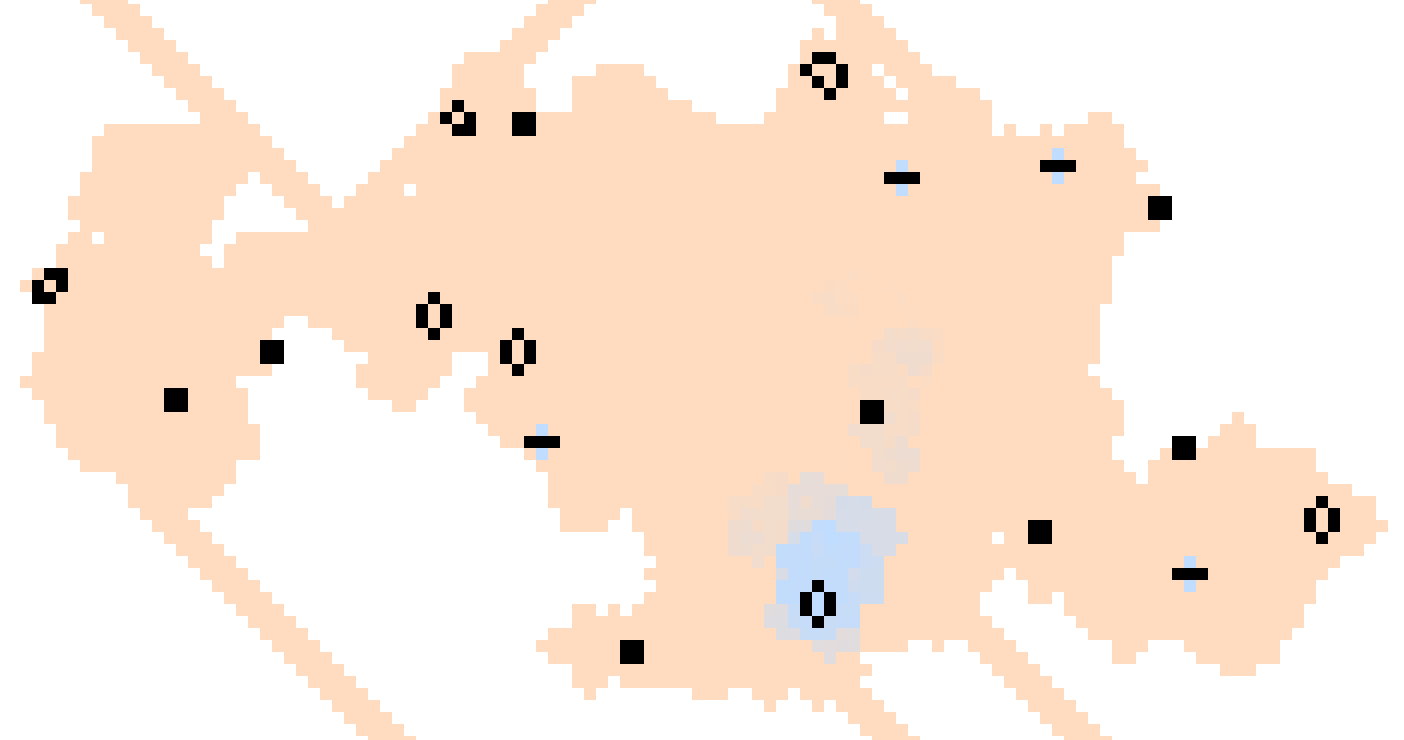
\includegraphics[scale=0.1]{early_life/r_pentomino_evolved}}}}
	\caption{An R-pentomino takes $1{\thousep}103$ generations to stabilize---much longer than any other polyomino with 5 or fewer cells. Along the way, it produces numerous other important patterns such as the \textbf{B-heptaplet} highlighted in \bgbox{aquaback}{aqua} and the \textbf{Herschel} highlighted in \bgbox{magentaback}{magenta}.}\label{fig:r_pentomino}
\end{figure}

We could similarly ask what the longest-lived pattern with $n$ cells for $n = 6, 7, 8, \ldots$ are. The longest-lived such patterns that are known are summarized in Table~\ref{tab:small_methuselahs}, as long as we restrict our attention only to patterns with reasonably small bounding boxes (which of course is subjective). However, these patterns are only known to be optimal for $n \leq 9$; the longest-lasting known $10$-cell methuselah in a small bounding box was not found until 2019, so above $n = 9$ there may still be new discoveries to be made.\footnote{Exhaustive computer searches for methuselahs with $n \leq 9$ cells were carried out by Paul Callahan in 1997, Tomas Rokicki in 2005, and Nick Gotts in 2019.}

\begin{table}[!htb]\vspace*{0.05in}
	\begin{center}		
		\begin{tabular}{Sc Sc Sl Sc}
			\toprule
			Cells & Methuselah & Name & Lifespan \\\midrule
			\specialcell{5} & \specialcell{\patternimglink{0.1}{5_cell_methuselahs}} & \specialcell{R-pentomino grandparents} & \specialcell{$1{\thousep}105$} \\
			
			\rowcolor{gray!20} \specialcell{6} & \specialcell{\patternimglink{0.1}{6_cell_methuselahs}} & \specialcell{R-pentomino great-great-great grandparents} & \specialcell{$1{\thousep}108$} \\
			
			\specialcell{7} & \specialcell{\patternimglink{0.1}{acorn}} & \specialcell{acorn\index{acorn}} & \specialcell{$5{\thousep}206$} \\
			
			\rowcolor{gray!20} \specialcell{8} & \specialcell{\patternimglink{0.1}{7468M}} & -- & \specialcell{$7{\thousep}468$} \\
			
			\specialcell{9} & \specialcell{\patternimglink{0.1}{bunnies}} & \specialcell{bunnies 9\index{bunnies!9}} & \specialcell{$17{\thousep}410$} \\ % bunnies 9
			
			\rowcolor{gray!20} \specialcell{10} & \specialcell{\patternimglink{0.1}{bunnies_10b}} & \specialcell{bunnies 10b\index{bunnies!10b}} & \specialcell{$17{\thousep}431$} \\ % bunnies 10b
			
			\specialcell{11} & \specialcell{\patternimglink{0.1}{23334M}} & -- & \specialcell{$23{\thousep}334$} \\
			
			\rowcolor{gray!20} \specialcell{12} & \specialcell{\patternimglink{0.1}{methuselah_12}} & -- & \specialcell{$23{\thousep}801$} \\
			
			\specialcell{13} & \specialcell{\patternimglink{0.1}{lidka}} & \specialcell{Lidka\index{Lidka}} & \specialcell{$29{\thousep}126$} \\\bottomrule
		\end{tabular}
		\caption{The longest-lived known methuselahs with 5--13 cells. The methuselahs with 7 or fewer cells were all known by no later than 1971: the R-pentomino relatives were fairly well-known, so their exact discoverer is difficult to pin down, but the acorn was found by Charles Corderman. The methuselah with 8 cells was found by Tomas Rokicki in 2005, bunnies~9 was found by Paul Callahan in 1997, bunnies 10b was found by Nick Gotts in November 2019, and the 11-, 12-, and 13-cell methuselahs were found by Simon Ekström in May 2016, February 2017, and March 2017, respectively.}\label{tab:small_methuselahs}
	\end{center}
\end{table}

To highlight the difficulty of defining methuselahs in a rigorous way, note that there are 8- and 9-cell patterns that can be made to have lifespans as long as we like, since we can just aim a glider at a far away blinker or a block. However, these somewhat trivial examples can be avoided by requiring that a methuselah have a suitably small bounding box (which also rules out $8$-cell methuselahs like the one displayed in Exercise~\ref{exer:8cell_methuselah}). If we go this route and focus on the bounding box of a pattern, rather than its number of cells, then we find patterns like the one displayed in Figure~\ref{fig:52513m},\footnote{Found by Dylan Chen in January 2021.} which fits within a $16 \times 16$ bounding box and has a lifespan of $52{\thousep}513$ generations, which is longer than any other known pattern of this size.

Another potential problem that arises when discussing methuselahs and stability comes from the fact that we already saw patterns with just 12 cells that grow indefinitely: the block-laying and glider-producing switch engines\footnote{This can easily be reduced to 11 cells by removing one of the cells in the block in either pattern.} of Section~\ref{sec:switch_engine}. This is not too difficult to take care of: even though these patterns grow forever, they do so in a regular and predictable way. For example, to know what a block-laying switch engine looks like in generation $5{\thousep}000{\thousep}000$, we don't actually need to evolve it $5{\thousep}000{\thousep}000$ times: we could simply move the switch engine the correct number of spaces to the northeast and paste a trail of blocks behind it. We could thus say, for example, that the block-laying switch engine stabilizes once it enters the periodic portion of its evolution where it repeatedly lays $8$ blocks every $288$ generations.

% This figure ideally should be 1 paragraph later.
\begin{figure}[!htb]
	\centering
	\begin{minipage}[b]{0.4\textwidth}
		\centering\patternimglink{0.11}{52513m}
		\caption{A methuselah that fits within a $16 \times 16$ bounding box and takes $52{\thousep}513$ generations to stabilize.}\label{fig:52513m}
	\end{minipage}\hfill
	\begin{minipage}[b]{0.56\textwidth}
		\centering\patternimglink{0.09}{ark_736692}
		\caption{A 16-cell pattern that takes a whopping $736{\thousep}692$ generations to stabilize. The $8$-cell objects at the top-right and bottom-left individually are just predecessors of the switch engine, so this pattern is an ark.}\label{fig:ark_736692}
	\end{minipage}
\end{figure}

These problems might seem simple enough to overcome by tweaking our definitions carefully, but they are just the tip of the iceberg when it comes to what can go wrong when trying to rigorously define methuselahs and what it means for a pattern to stabilize. As yet another example, consider the remarkable 16-cell pattern\footnote{Found by Nick Gotts in 2005.} depicted in Figure~\ref{fig:ark_736692}, which takes $736{\thousep}692$ generations to stabilize.

The ``problem'' with this pattern is that its non-stabilization is rather artificial; it evolves into adjacent block-laying and glider-producing switch engines, which interact in such a way as to fire a glider backward toward some debris every $2{\thousep}304$ generations. Every time this backward glider hits the debris, it transforms it into something slightly different and unpredictable. This process repeats more than 250 times before it breaks down and a glider destroys the debris enough that future gliders pass right through without touching it at all. However, by this point the pattern has been growing for over $700{\thousep}000$ generations into the huge mess shown in Figure~\ref{fig:ark_736692_stabilized}.

\begin{figure}[!htb]
	\centering\begin{tikzpicture}%
	\node[inner sep=0pt,anchor=south west] (zoom1) at (-1,1) {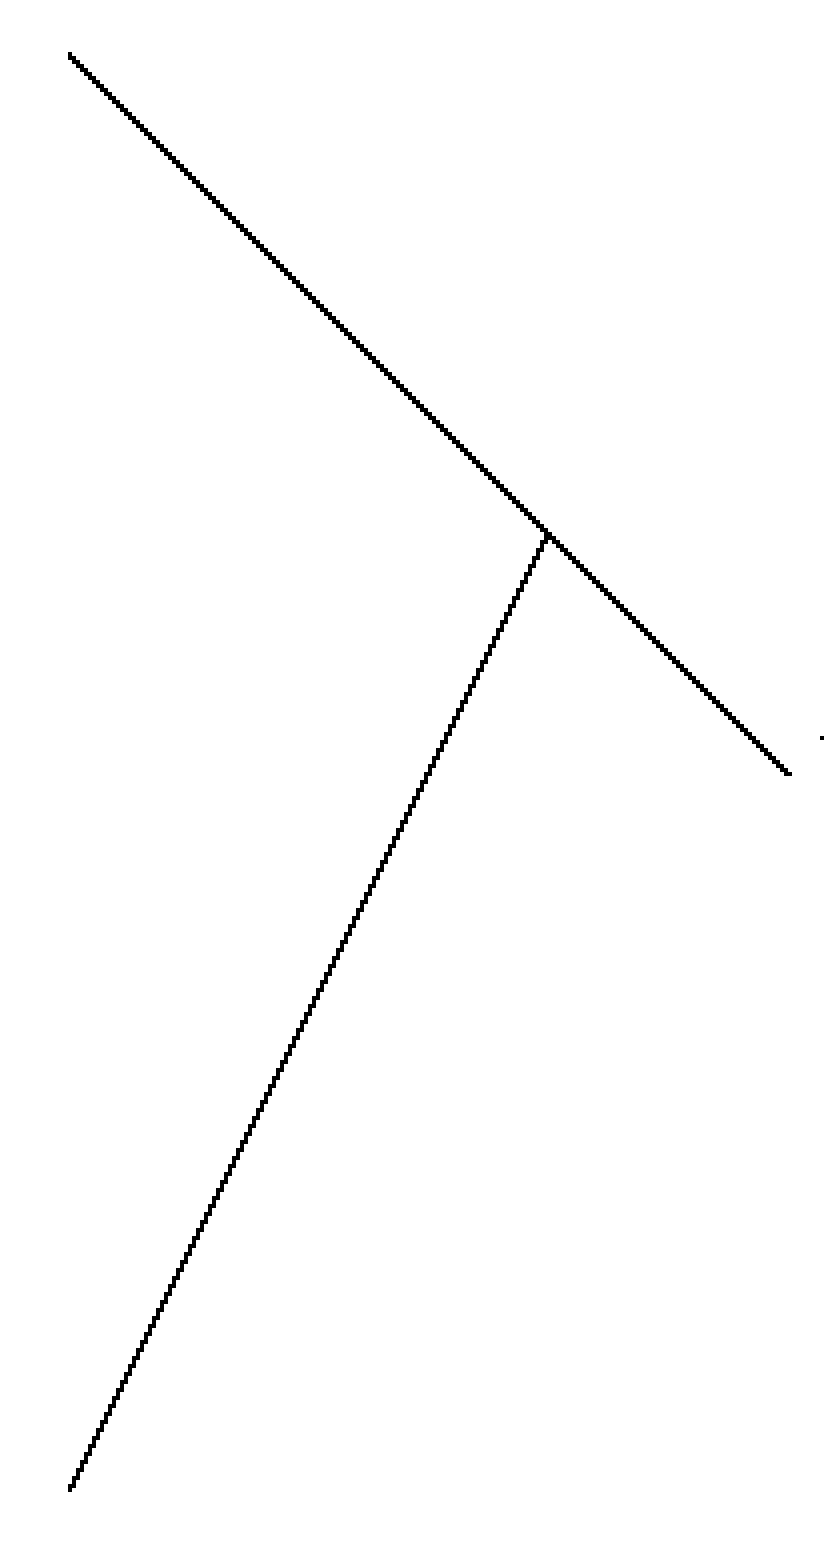
\includegraphics[width=2.8cm]{early_life/ark_736692_1.png}};
	\draw[gridgray,line width=0.75pt] (-1,1) rectangle (1.8,6.147);
	
	% ZOOM BOX 1
	\path[draw,gridgray,line width=0.5pt] (1.653,3.803) -- (11.9,8.1) -- cycle;
	\path[draw,gridgray,line width=0.5pt] (1.653,3.55) -- (11.9,0) -- cycle;
	
	\path[fill,white,opacity=0.85,line width=0pt] (1.4,3.55) -- (3.8,0) -- (11.9,0) -- (11.9,8.1) -- (3.8,8.1) -- (1.4,3.803) -- (1.653,3.803) -- (1.653,3.55) -- cycle;
	\draw[gridgray,line width=0.5pt] (1.4,3.55) rectangle (1.653,3.803);
	
	\path[draw,gridgray,line width=0.5pt] (1.4,3.803) -- (3.8,8.1) -- cycle;
	\path[draw,gridgray,line width=0.5pt] (1.4,3.55) -- (3.8,0) -- cycle;
	
	\node[inner sep=0pt] (zoom1_32x) at (2.8,3.7) {
\includegraphics[width=0.3cm]{mag.png} 32x};
	% END ZOOM BOX 1
	
	\node[inner sep=0pt,anchor=south west] (zoom2) at (3.8,0) {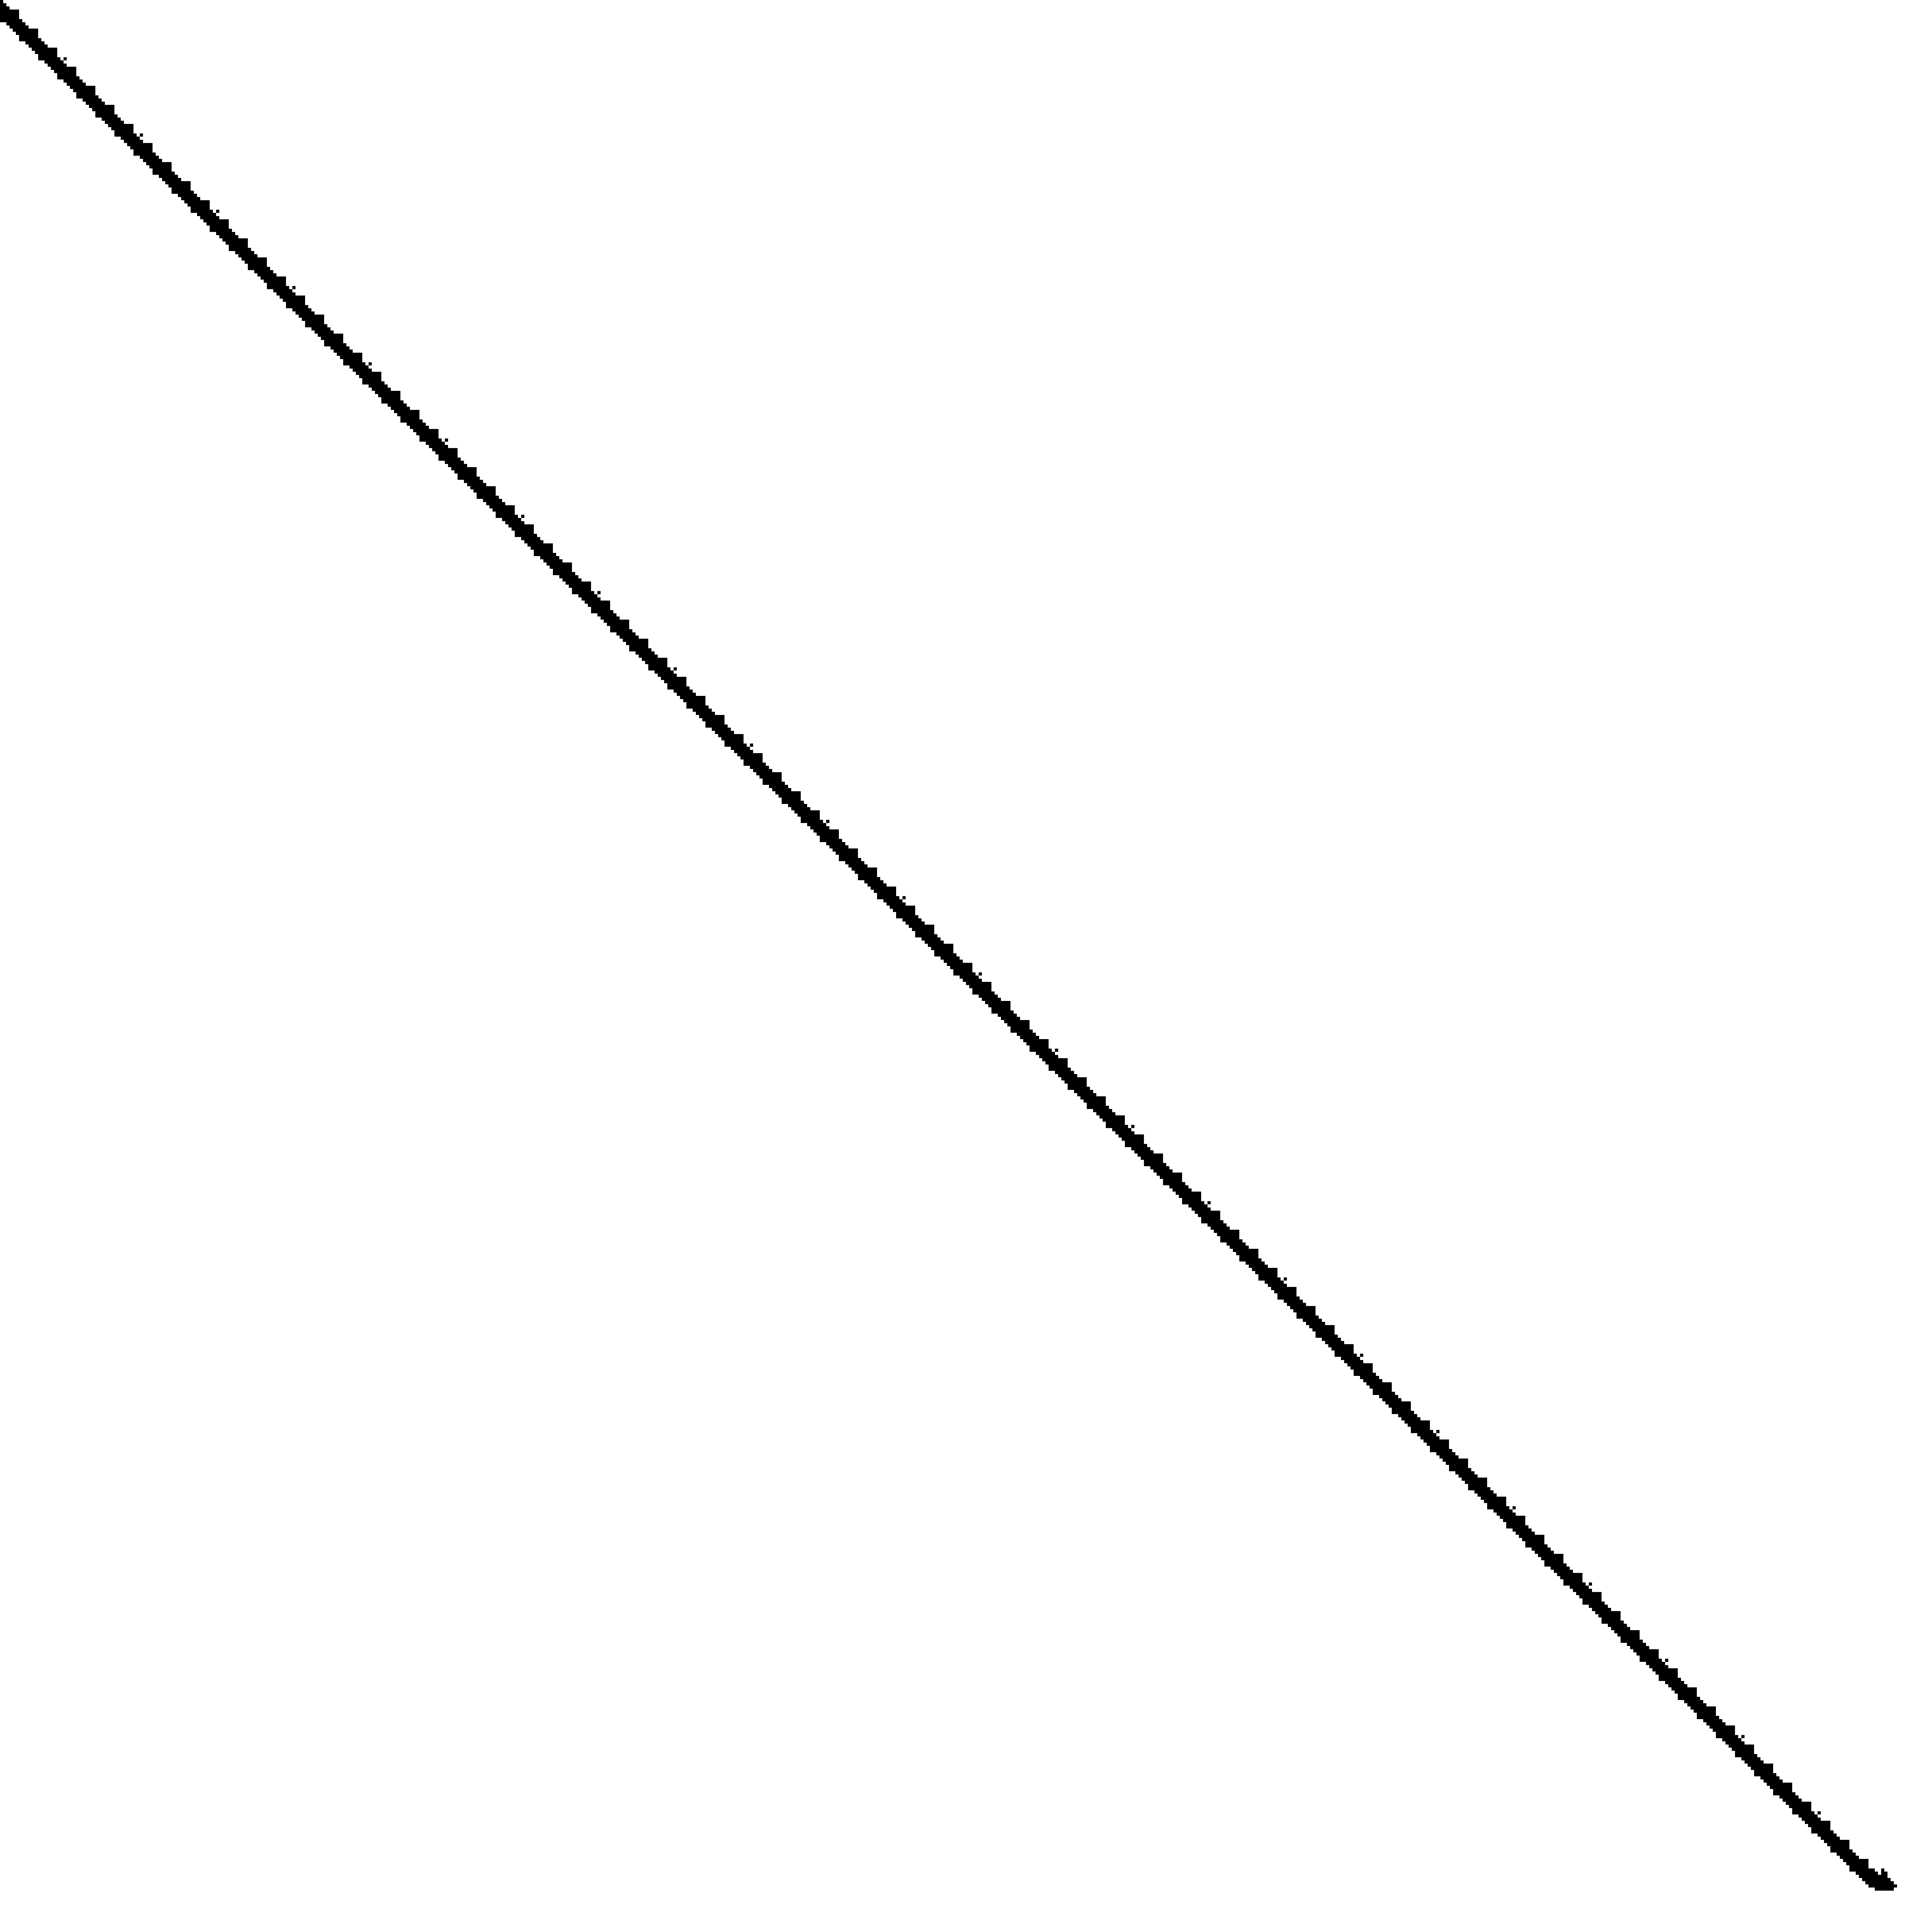
\includegraphics[width=8.1cm]{early_life/ark_736692_2.png}};
	\draw[gridgray,line width=0.75pt] (3.8,0) rectangle (11.9,8.1);
	
	% ZOOM BOX 2
	\path[draw,gridgray,line width=0.5pt] (11.51,0.14) -- (2,-9) -- cycle;
	
	\path[fill,white,opacity=0.85,line width=0pt] (11.51,0.367) -- (2,-1.75) -- (2,-9) -- (10.53,-9) -- (11.777,0.14) -- (11.51,0.14) -- cycle;
	\draw[gridgray,line width=0.5pt] (11.51,0.14) rectangle (11.777,0.367);
	
	\path[draw,gridgray,line width=0.5pt] (11.51,0.367) -- (2,-1.75) -- cycle;
	\path[draw,gridgray,line width=0.5pt] (11.777,0.367) -- (10.53,-1.75) -- cycle;
	\path[draw,gridgray,line width=0.5pt] (11.777,0.14) -- (10.53,-9) -- cycle;
	
	\node[inner sep=0pt] (zoom1_32x) at (9,-1) {
\includegraphics[width=0.3cm]{mag.png} 32x};
	% END ZOOM BOX 2
	
	\node[inner sep=0pt,anchor=south west] (zoom3) at (2,-9) {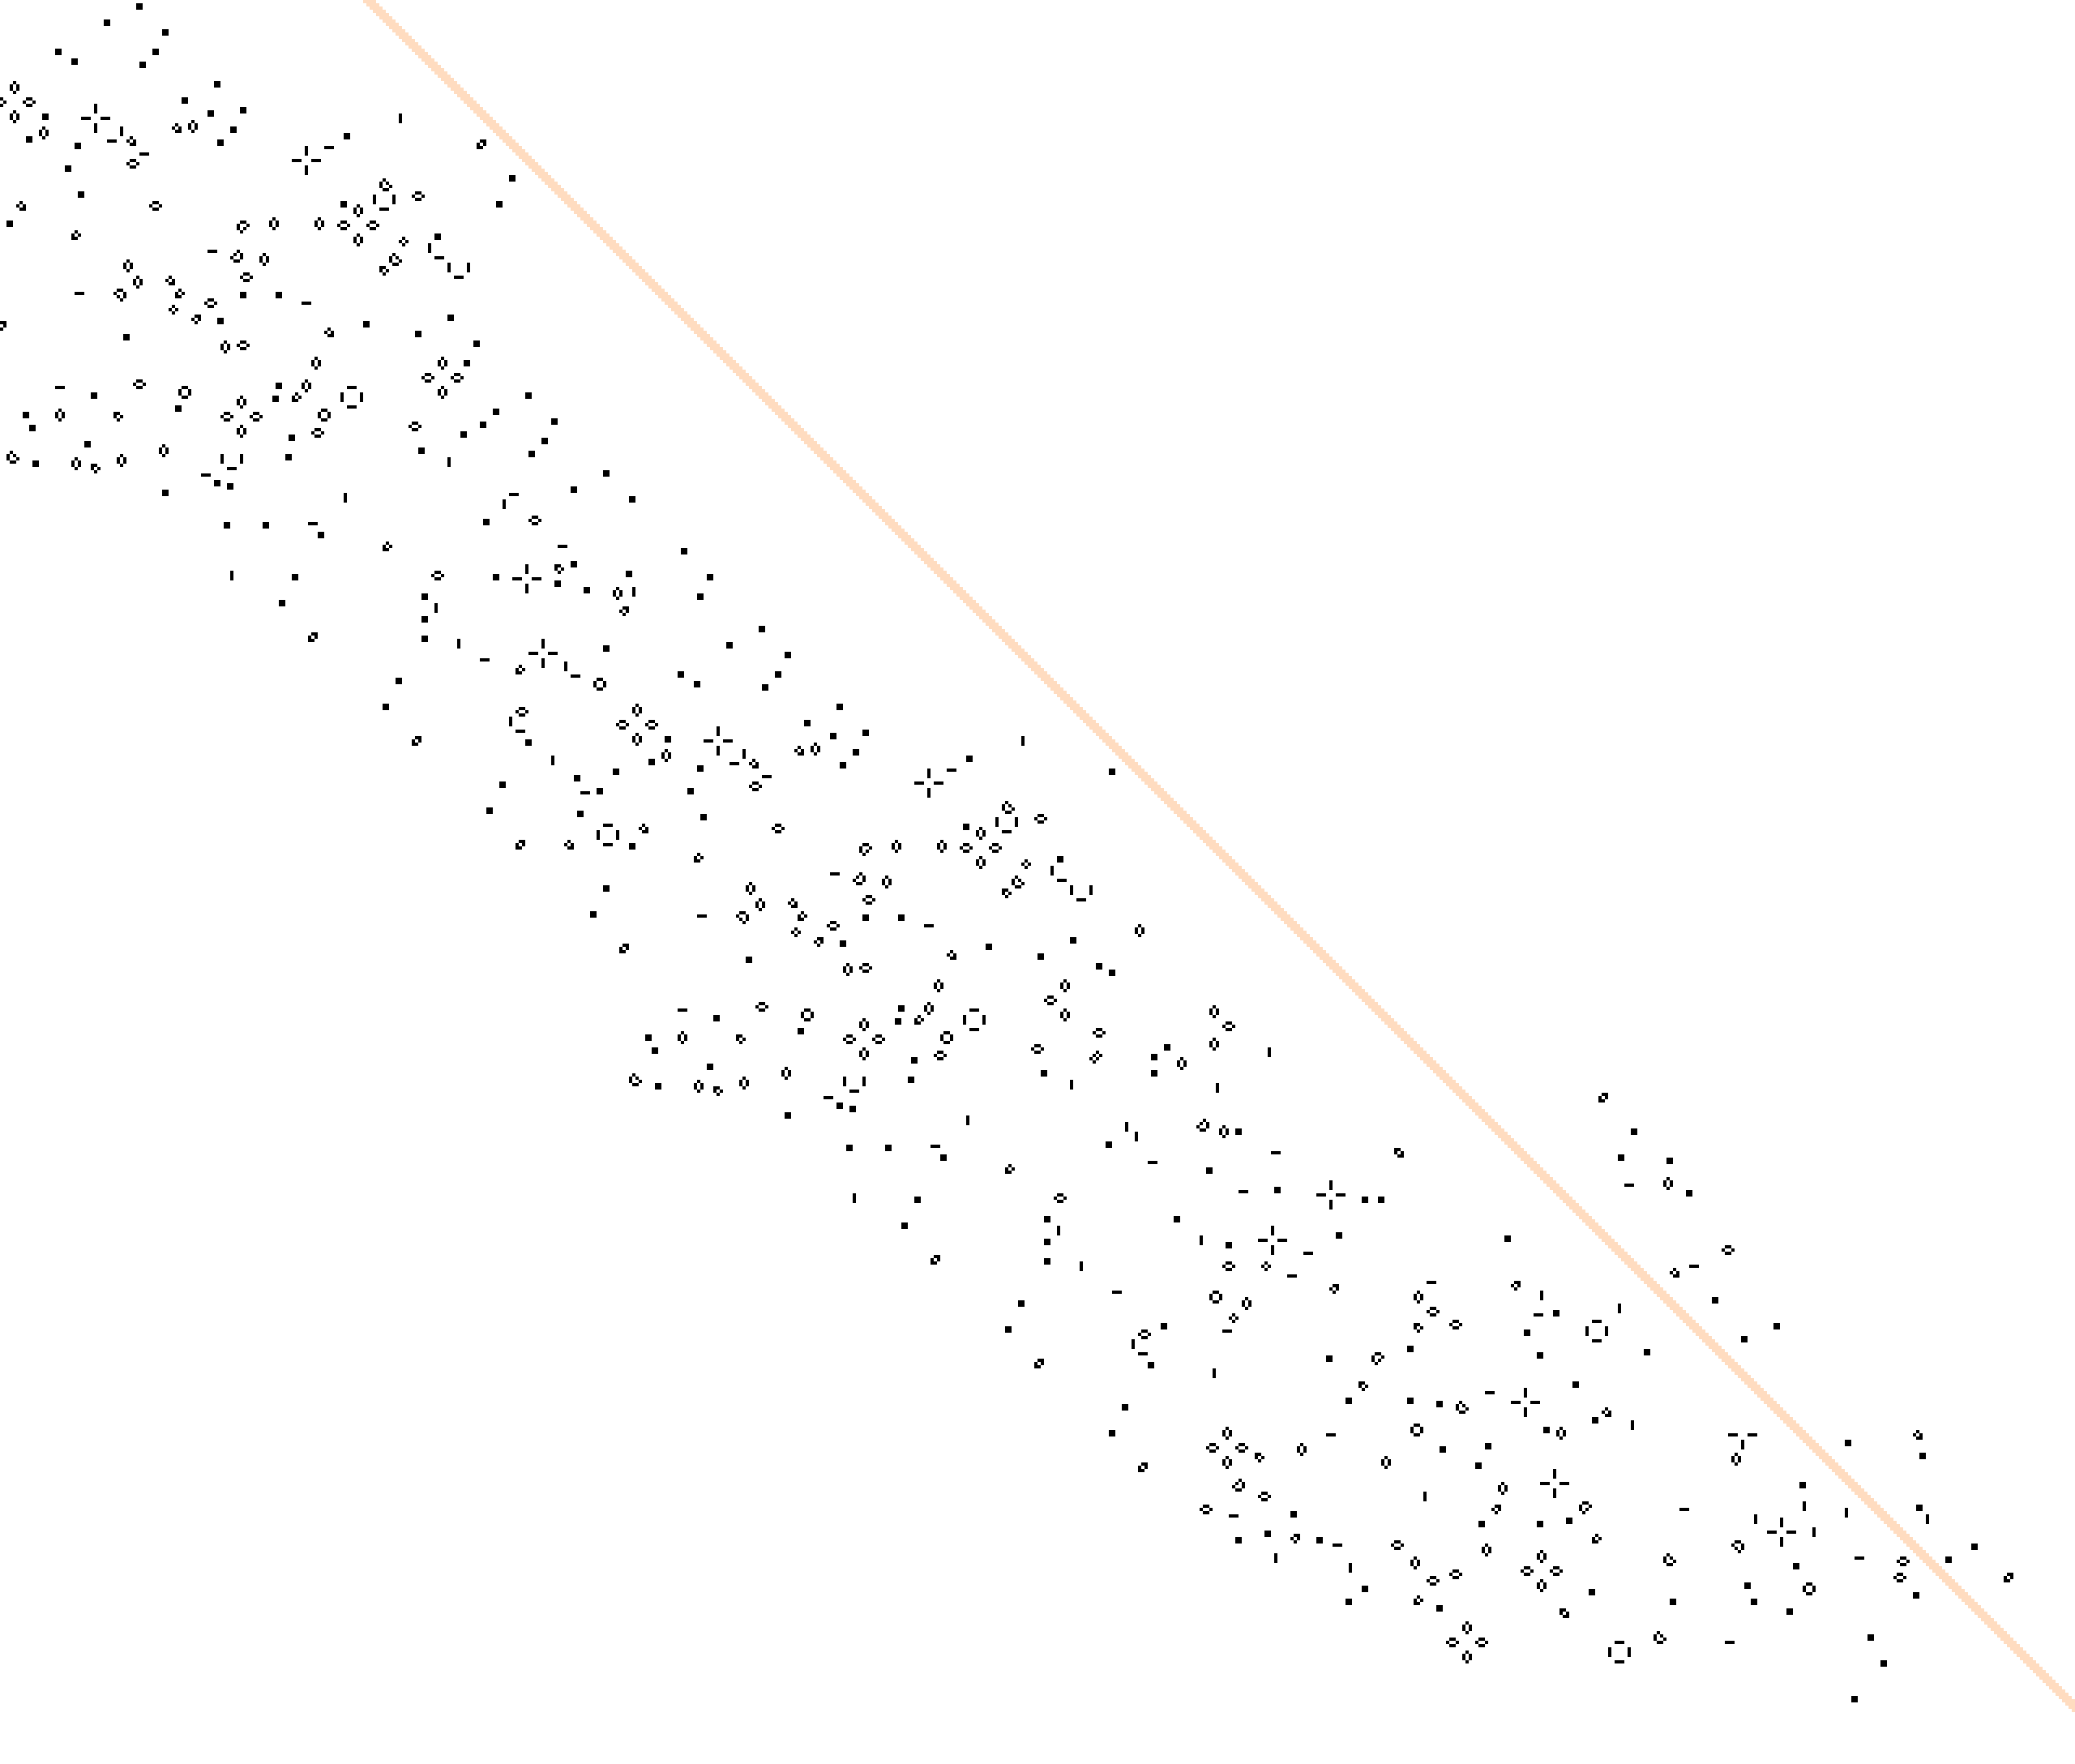
\includegraphics[width=8.53cm]{early_life/ark_736692_3.png}};
	\draw[gridgray,line width=0.75pt] (2,-9) rectangle (10.53,-1.75);
	\end{tikzpicture}
	
	\caption{The pattern from Figure~\ref{fig:ark_736692} leaves behind this absolutely massive ash after $736{\thousep}692$ generations. We have zoomed in by a factor of $32 \times 32 = 1{\thousep}024$ on the corner of the ash that the pattern started growing from, which is also the corner that contains the debris that gliders are fired at throughout its extensive lifespan. The \bgbox{orangeback2}{orange} line on the bottom-right depicts the southeastward path taken by gliders that now (just barely) miss hitting the debris.}\label{fig:ark_736692_stabilized}
\end{figure}

While patterns like this one are certainly interesting, they are not quite in the spirit of what we want from methuselahs---even though the previous pattern did not completely stabilize for hundreds of thousands of generations, it was ``mostly'' stable for the vast majority of that time. Rather, we would like methuselahs to take a long time to stabilize based primarily on chaos that we cannot completely break down into simple reactions like gliders repeatedly hitting some debris. We will not try to make this precise, but rather just leave it as a phenomenon that we know when we see.

To briefly suggest some even more extreme examples of the weirdness that happens with stability, note that we will learn in Chapter~\ref{chp:periodic_circuitry} how to construct a pattern that computes the prime numbers. Should such a pattern be considered stable? Perhaps even more striking than this, in Section~\ref{sec:unknown_growth} we will then create a pattern whose long-term behavior we do not understand: it might continue to grow in a reasonably regular fashion indefinitely, or it might stabilize into a finite pattern. What we do know is that it continues to grow for at least its first $10^{2{\thousep}500{\thousep}000{\thousep}000}$ generations, so if it does eventually stabilize and remain finite, it must do so after that point (and we have no hope of actually simulating the pattern long enough to find out the answer).

Even worse than this, in Chapter~\ref{chp:universal_computation} we will demonstrate how to construct patterns that compute anything that can be computed by a computer. We can thus encode a huge variety of unsolved mathematical and computational problems into Life patterns, many of which have long-term behavior that we have absolutely no hope of determining.


%%%%%%%%%%%%%%%%%%%%%%%%%%%%%%%%%%%%%%%%%%%%%%%%%%%%%%%%%%%%%%%%%%%%%%%%%
%%   SECTION: GARDENS OF EDEN
%%   http://wwwhomes.uni-bielefeld.de/achim/orphan.html
%%%%%%%%%%%%%%%%%%%%%%%%%%%%%%%%%%%%%%%%%%%%%%%%%%%%%%%%%%%%%%%%%%%%%%%%%
\section{Gardens of Eden}\label{sec:goe}\index{Garden of Eden}

Oftentimes, a lot can be learned by considering Life in reverse: instead of investigating what a pattern evolves into, we investigate what evolves into it. That is, we look for parents (and grandparents, and great-grandparents, ...) of the pattern that we are interested in.\footnote{Strictly speaking, if a pattern has one parent then it must have infinitely many, since we could just add any pattern that dies in one generation far away. When discussing how many parents a pattern has, we will always ignore parents that have dying ash like this that has no effect on their evolution.} Some patterns, such as the block, have numerous parents (see Figure~\ref{fig:block_parents}), which is part of the reason why they appear so frequently in the ash of random soups.

\begin{figure}[!htb]
	\centering\patternimglink{0.1}{block_parents}
	\caption{Six small parents of the block. From left-to-right, the first three of these objects are the block\index{block}, \textbf{pre-block}\index{pre-block}, and \textbf{grin}\index{grin}, respectively, while the other three do not have names.}\label{fig:block_parents}
\end{figure}

Other patterns, such as the clock\index{clock}, have relatively few parents and thus appear less frequently in random soups. Recall that the clock has only six cells and is period~2. Surprisingly, it appears in random soups much less frequently than some much larger objects like the period~3 pulsar or the period~15 pentadecathlon. It seems natural to ask whether or not there exists a pattern that does not have even a single parent. That is, does there exist a pattern that cannot ever appear in the evolution of any other pattern, but rather can only ever appear in generation~$0$?\footnote{Generation~$0$ refers to the starting configuration, before applying the Life rules to it. Generation~$1$ is the pattern that is obtained by applying the Life rules once, and generation~$n$ is the pattern obtained by applying the Life rules $n$ times.} A pattern with this property is called a \textbf{Garden of Eden},\footnote{This term was coined in the context of cellular automata by John W. Tukey in the 1950s, long before Conway's Game of Life was introduced.} and we begin by showing that they do indeed exist.

The rough idea of why Gardens of Eden must exist is that some patterns (such as blocks) have lots of parents, so there are not enough parents left over for all other patterns. To prove this explicitly, we will barely need to use anything more than the fact that blocks and pre-blocks both evolve into the same thing.\footnote{We could instead use two other objects that evolve into the same thing in the proof: we just use blocks and pre-blocks because they are so simple.}	

\begin{theorem}[Existence of Gardens of Eden]\label{thm:garden_of_eden_exists}
	There exist Gardens of Eden in Conway's Game of Life.
\end{theorem}

\begin{proof}
	Let $n \geq 1$ be an integer and consider all patterns that fit within a $6n \times 6n$ square on the Life grid. The contents of the central $(6n-2) \times (6n-2)$ square in generation~1 only depend on the contents of the original $6n \times 6n$ square in generation~0. This central $(6n-2) \times (6n-2)$ square contains $(6n-2)^2$ cells, each of which can be alive or dead, so there are $2^{(6n-2)^2}$ distinct patterns that could fill this central square. We will now show that, if $n$ is large enough, some of these patterns must have no parent.
	
	\begin{figure}[!htb]
		\centering\patternimg{0.1}{goe_theorem_tiles}
		\caption{Two $6 \times 6$ tiles that evolve the same way no matter what is placed outside of the tiles.}\label{fig:goe_theorem_tiles}
	\end{figure}
	
	To this end, partition the $6n \times 6n$ square into $n^2$ tiles, each of size $6 \times 6$. Each tile contains $36$ cells, each of which can be alive or dead, so there are $2^{36}$ different tiles. However, the two tiles displayed in Figure~\ref{fig:goe_theorem_tiles} evolve in the same way regardless of what other tiles are placed around them. We thus conclude that in any pattern that uses the first tile, we could replace it by the second tile without changing the evolution of the overall pattern (see Figure~\ref{fig:goe_theorem_tiles_example}). It follows that if we want to catalog all possible patterns that can be present in generation~$1$, we only need to consider patterns made up of one of $2^{36} - 1$ (not $2^{36}$) different tiles in generation~$0$.
	
	\begin{figure}[!htb]
		\centering\patternimglink{0.1}{goe_theorem_tiles_example}
		\caption{A $6n \times 6n$ pattern in the $n = 4$ case, broken down into $6 \times 6$ tiles. Each of the tiles containing only a block in the center (outlined in \bgbox{aquaback}{aqua}) can be replaced by a tile with a pre-block in the center without affecting the evolution of the overall $24 \times 24$ pattern.}\label{fig:goe_theorem_tiles_example}
	\end{figure}
	
	Since the $6n \times 6n$ square has $n^2$ of these tiles, there are at most $(2^{36}-1)^{n^2}$ different possible children (i.e., patterns present in generation~$1$). Since there are $2^{(6n-2)^2}$ distinct patterns that could fill the central $(6n-2) \times (6n-2)$ square, but at most $(2^{36}-1)^{n^2}$ of them appear in children of patterns in the $6n \times 6n$ square, all that remains is show that $(2^{36}-1)^{n^2} < 2^{(6n-2)^2}$ when $n$ is sufficiently large. Taking the $n^2$-th root of both sides of the inequality reduces it to $2^{36} - 1 < 2^{(6 - 2/n)^2}$, which is indeed true when $n$ is sufficiently large, since we can make $2/n$ arbitrarily close to $0$ and hence $2^{(6 - 2/n)^2}$ arbitrarily close to $2^{6^2} = 2^{36}$ (in particular, we can make it larger than $2^{36} - 1$).\footnote{In fact, not only is it the case that $(2^{36}-1)^{n^2} < 2^{(6n-2)^2}$ when $n$ is large, but the ratio $(2^{36}-1)^{n^2} / 2^{(6n-2)^2}$ can be made as small as we like by making $n$ sufficiently large (see Exercise~\ref{exer:goe_theorem_limit}). In other words, not only do Gardens of Eden \emph{exist}, but in fact almost all large patterns are Gardens of Eden.}
\end{proof}

It is worth noting that the method used in the proof of Theorem~\ref{thm:garden_of_eden_exists} is very general and applies to any cellular automaton for which two distinct (finite) patterns evolve into the same pattern.\footnote{This more general theorem was proved by Edward F. Moore and John Myhill in the early 1960s \cite{Moo62,Myh63}, so Gardens of Eden were known to exist in Conway's Game of Life right from the moment it was introduced.} Also, even though it is non-constructive, it can be used to find (extremely loose) bounds on how large Gardens of Eden must be---see Exercise~\ref{exer:goe_theorem}.

Now that we know that Gardens of Eden exist, our next goal is to actually find an explicit example of one.\footnote{The first explicit Garden of Eden in the Game of Life was constructed by Roger Banks in 1971.} Unfortunately, our method of proof of Theorem~\ref{thm:garden_of_eden_exists} is not of much help here, since it only shows that Gardens of Eden exist in extremely large regions (the smallest $n$ for which the inequality $(2^{36}-1)^{n^2} < 2^{(6n-2)^2}$ holds is somewhere around $n \approx 10^{12}$), and it does not actually tell us how to find one in such a region. The pattern obtained by concatenating together all $2^{n^2}$ different $n \times n$ patterns into a rectangle of size $2^{n^2} n \times n$ is guaranteed to be a Garden of Eden, but it is exponentially larger than the upper bound provided by the theorem.

Our method of construction is to build a Garden of Eden one cell at a time, repeatedly choosing the new cell that we add to the pattern so as to result in it having as few parents as possible. More explicitly, we build this Garden of Eden as follows:\footnote{This method is due to Nicolay Beluchenko \cite{A196447}.}\medskip

\begin{itemize}
	\item We consider the two possible states of a single cell. Out of the $2^9 = 512$ possible configurations of the $3 \times 3$ square centered at this cell, $372$ lead to the central cell being dead and $140$ lead to it being alive. Thus we make that central cell alive, so as to have fewer parents.\smallskip
	
	\item We then consider the two possible states of a cell that is adjacent to the starting (alive) cell. Out of the $140 \times 2^3 = 1{\thousep}120$ possible configurations of the $4 \times 3$ rectangle centered at those two cells that lead to the first cell being alive, $703$ lead to the second cell being dead and $417$ lead to it being alive. We thus make the second cell alive, so as to have fewer parents.\smallskip
	
	\item We continue in this way in a clockwise spiral around the initial cell, deciding whether each new cell will be alive or dead based on which of the two possibilities results in a pattern with fewer parents.\medskip
\end{itemize}

While this method might seem not to yield anything useful at first---after 40 cells, each of them has been chosen to be alive, and the number of parents has exploded to $4{\thousep}624{\thousep}592$---the number of parents does eventually start to dwindle, and after 266 cells the pattern has no parents at all (and is thus a Garden of Eden).\footnote{In step 262 there is a tie between the number of parents if the cell is chosen to be alive or dead. We (arbitrarily) chose the cell to be alive.} This Garden of Eden is displayed in Figure~\ref{fig:goe_1}.

\begin{figure}[!htb]
	\centering\begin{tikzpicture}%
	\node[inner sep=0pt,anchor=south west] at (0,0) {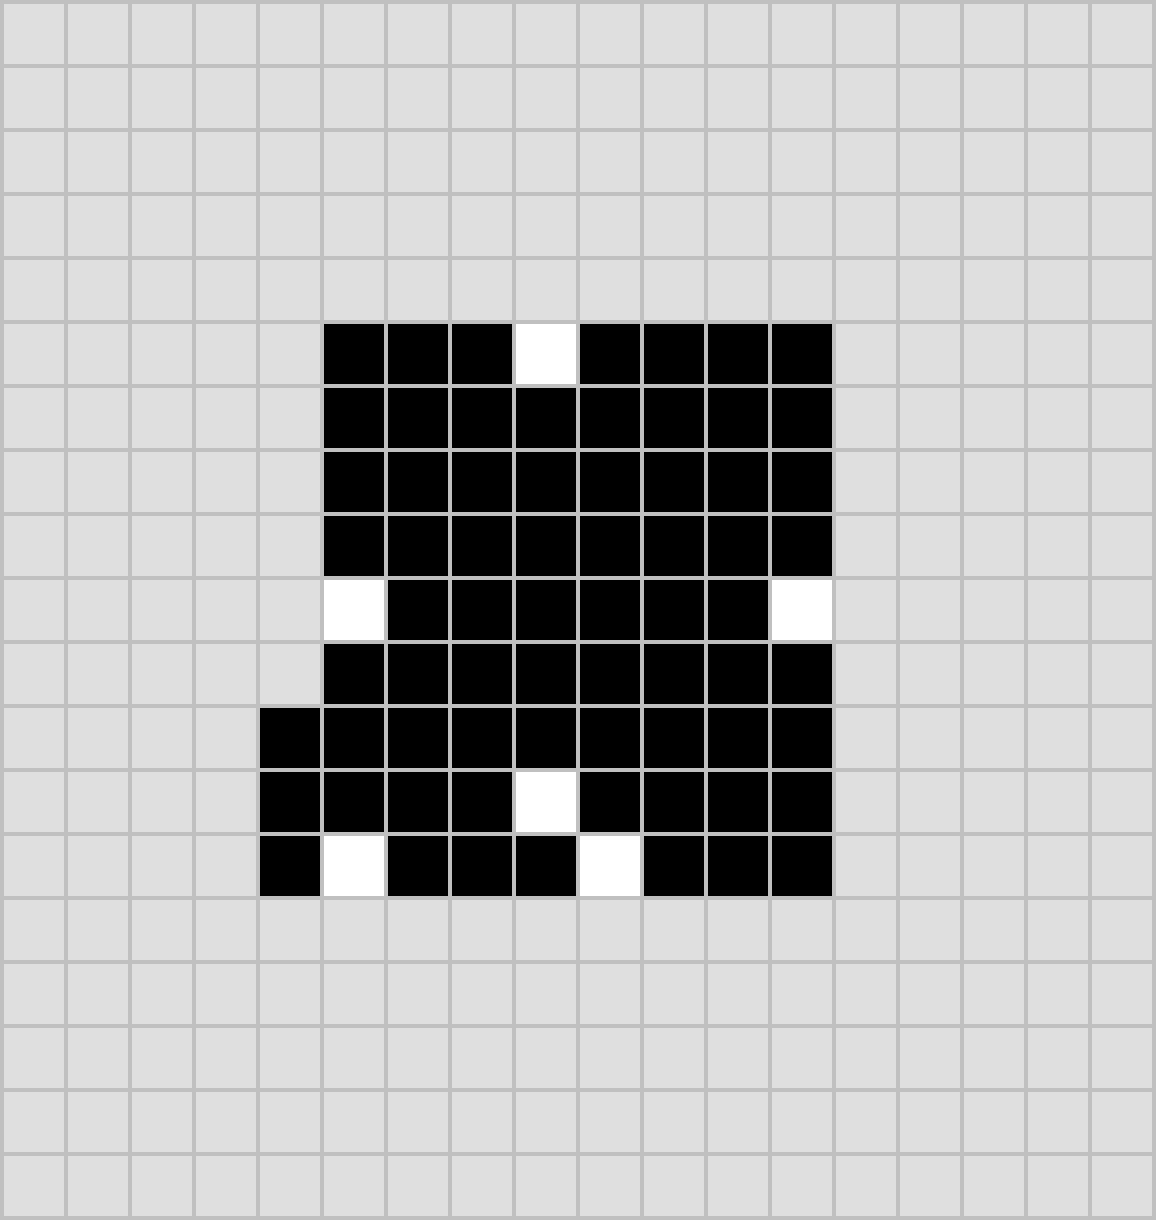
\includegraphics[width=4cm]{early_life/goe_1_partial.png}};
	\draw[->][black,line width=1pt] (1.02,1.88) -- (1.02,3.22) -- (2.4,3.22);
	
	\node[inner sep=0pt,anchor=south west] at (6,0) {\embedlink{goe_1}{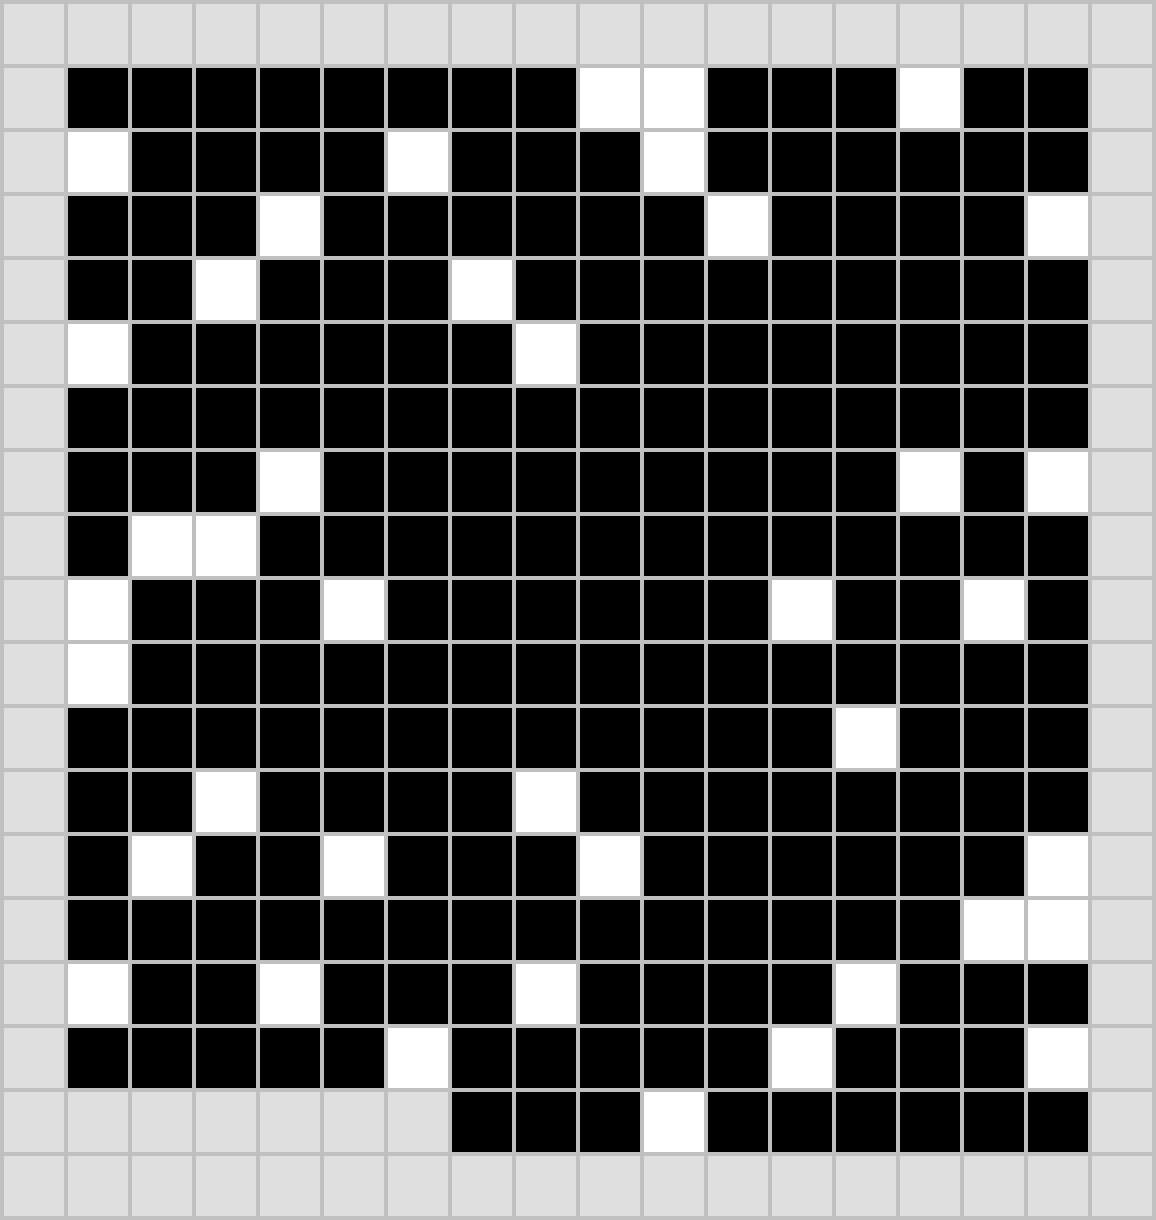
\includegraphics[width=4cm]{early_life/goe_1.png}}};
	\end{tikzpicture}
	
	\caption{A partial Garden of Eden (left) that is being constructed one cell at a time by placing cells in a clockwise spiral, choosing whether they should be alive or dead based on which state results in fewer parents. The completed Garden of Eden (right) has 41 dead cells and 225 alive cells (the \bgbox{gridgray!40}{light gray} cells are unspecified---the pattern remains a Garden of Eden regardless of whether they are alive or dead).}\label{fig:goe_1}
\end{figure}

The pattern that we have constructed is interesting for the fact that it is not only a Garden of Eden, but it remains a Garden of Eden regardless of which live and dead cells we place outside of the central 266-cell spiral. Patterns like this one that cannot be \emph{any} part of the evolution of another pattern (equivalently, they are still a Garden of Eden no matter what other cells are placed around them) are called \textbf{orphans}\index{orphan}.\footnote{This term was coined by Conway. Also, the proof of Theorem~\ref{thm:garden_of_eden_exists} actually demonstrates the existence of orphans, not just Gardens of Eden.} Every pattern containing an orphan is (by definition) a Garden of Eden, and remarkably the converse is also true---every Garden of Eden contains an orphan.\footnote{This equivalence follows immediately from standard results in dynamical systems (see \cite{Hed69}, for example). It was made explicit by Jarkko Kari no later than 2010---see \httpsurl{conwaylife.com/forums/viewtopic.php?p=51782\#p51782}.}

Now that we know that small Gardens of Eden (and orphans) exist, we would like to know how small and simple they can be. A complete answer to this problem is still open (and perhaps is currently one of the most actively researched problems in Life), but many partial results are known. The smallest known orphans and Gardens of Eden (in terms of number of cells and bounding box size) are presented in Figure~\ref{fig:goe_records}.\footnote{These patterns can be verified to be orphans via a computer program called \emph{JavaLifeSearch}---see \httpsurl{conwaylife.com/wiki/JavaLifeSearch} and Exercise~\ref{exer:goe_jls}.}\index{JavaLifeSearch}

\begin{figure}[!htb]
	\centering
	\begin{subfigure}{.31\textwidth}
		\centering
		\patternimglink{0.1}{goe_record_alive}
		\caption{An orphan with 45~live cells, found by Nicolay Beluchenko in 2009.}
		\label{fig:goe_record_alive}
	\end{subfigure} \ \ \ \ % 
	\begin{subfigure}{.31\textwidth}
		\centering
		\patternimglink{0.1}{goe_record_orphan}
		\caption{An orphan with 88~specified cells, found by Steven Eker in 2017.} % No longer cited? \cite{HHKN11}
		\label{fig:goe_record_orphan}
	\end{subfigure} \ \ \ \ % 
	\begin{subfigure}{.31\textwidth}
		\centering
		\patternimglink{0.1}{goe_record_bb}
		\caption{An orphan in a bounding box with area $96 = 8 \times 12$, found by Steven Eker in 2016.}
		\label{fig:goe_record_bb}
	\end{subfigure}
	\caption{The current smallest-known orphans by (a)~number of live cells, (b)~total number of live and dead cells specified, and (c)~bounding box area.}\label{fig:goe_records}
\end{figure}

On the other hand, there are also results that show that orphans cannot be ``too'' small. For example, exhaustive computer searches have shown that there does not exist an orphan that fits within a $6 \times 7$ bounding box.\footnote{This computation was carried out independently by Steven Eker and Marijn Heule in 2016.} In a similar vein, we now show that there does not exist a Garden of Eden (and thus there does not exist an orphan) that has a bounding box with height one.\footnote{This theorem was originally proved by Jean Hardouin--Duparc in 1974 \cite{Har74}.}

\begin{theorem}[No Thin Gardens of Eden]\label{thm:1_row_goe}
	In Conway's Game of Life, every pattern that fits within a bounding box of height~$1$ has a parent. In other words, there do not exist Gardens of Eden with height~$1$.
\end{theorem}

\begin{proof}
	We prove the theorem by explicit construction: we show how to find a parent of any $1$-cell-thick pattern. The key step in our construction is to build a border that dies off completely in one generation and guarantees that any junk placed inside of it does not expand outward in that generation. Figure~\ref{fig:1_row_border} shows one such border: no matter what we place inside the $3 \times n$ box in the middle of the border, no cell outside of that $3 \times n$ box will be alive in the next generation.
	
	\begin{figure}[!htb]
		\centering\patternimglink{0.12}{1_row_border}
		\caption{A border that can be used to help construct parents of 1-cell-thick patterns. No matter what we place in the central $3 \times n$ region, no cell outside of the $3 \times n$ region will be alive in the next generation. We will fill it in such a way so that the desired $1 \times (n-2)$ pattern evolves in the center row, highlighted in \bgbox{aquaback}{aqua}).}\label{fig:1_row_border}
	\end{figure}
	
	To complete the proof, we just need to find a way to fill that $3 \times n$ box in such a way that it evolves into any $1 \times (n-2)$ pattern that we desire. One simple method that \emph{almost} works is to put the desired pattern itself in the central row of the $3 \times n$ box, and its negation (i.e., flip all alive cells to dead and vice-versa) in the top and bottom rows of the $3 \times n$ box. It is straightforward to check that the cells in the top and bottom rows of the $3 \times n$ box will always be overpopulated, and thus those two rows will always be dead in the next generation. Furthermore, the central row evolves in the correct way in 7 out of every 8 possible configurations of three adjacent alive/dead cells (see Figure~\ref{fig:1_row_3x3}).
	
	\begin{figure}[!htb]
		\centering
		\begin{minipage}[b]{0.64\textwidth}
			\centering\begin{tikzpicture}[scale=1.1, every node/.style={transform shape}]%
			\fill[color=redback] (2.2,0.95) rectangle (3.25,-1.35);
			\fill[color=yellowback2] (6.8,0.95) rectangle (7.85,-1.35);
			\node[inner sep=0pt,anchor=south west] at (0,0) {\patternimg{0.102}{1_row_3x3}};
			\node[inner sep=0pt,anchor=south west] at (0.3,-0.52) {$\downarrow \qquad \ \ \downarrow \qquad \ \ \downarrow \qquad \ \ \downarrow \qquad \ \ \downarrow \qquad \ \ \downarrow \qquad \ \ \downarrow \qquad \ \ \downarrow$};
			\node[inner sep=0pt,anchor=south west] at (0.23,-1.1) {\patternimg{0.102}{1_row_3x3_evolved}};
			\end{tikzpicture}
			\caption{All except for one of the $8$~different $3 \times 3$ squares (the one highlighted in \bgbox{redback}{red}) in which the top and bottom rows are the negation of the middle row evolve so that the top and bottom rows die and the middle cell stays the same.}\label{fig:1_row_3x3}
		\end{minipage}\hfill\begin{minipage}[b]{0.32\textwidth}
			\centering\gridbox{1pt}{\begin{tikzpicture}[scale=0.5, every node/.style={transform shape}]%
				\node[inner sep=0pt,anchor=south west] (glider_loop) at (0.5,0.5) {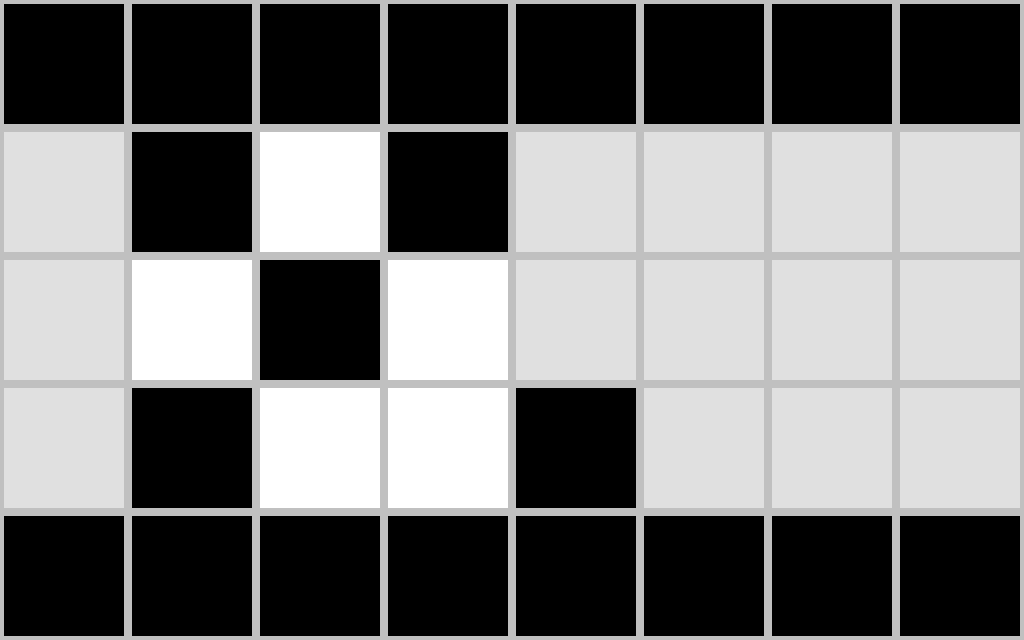
\includegraphics[width=8cm]{early_life/goe_1_row_proof.png}};
				%\draw[black!20,line width=2pt] (0,0) rectangle (5,-5);
				
				\letternode{4}{2}{A}
				\letternode{5}{2}{B}
				
				\letternode{5}{3}{X}
				\letternode{6}{3}{Y}
				\letternode{7}{3}{Z}
				\end{tikzpicture}}
			\caption{In order to correct the problematic $3 \times 3$ block from Figure~\ref{fig:1_row_3x3}, we set cell~A to be dead and cell~B to be alive, regardless of the state of cell~X.}\label{fig:goe_row_1_proof}
		\end{minipage}
	\end{figure}
	
	As a first attempt at fixing the problem that occurs when a single alive cell is between two dead cells in the middle row, simply set the bottom-right cell (i.e., cell~A in Figure~\ref{fig:goe_row_1_proof}) of that $3 \times 3$ block as dead, rather than alive. To compensate for this cell being dead, we also set the cell to its immediate right (i.e., cell~B in that figure) to be alive, regardless of whether cell~X is alive or dead. This corrects the evolution of the problematic $3 \times 3$ arrangement highlighted in red in Figure~\ref{fig:1_row_3x3}: the central cell in this $3 \times 3$ block now stays alive (since it now has exactly 3 live neighbors) and the cell to its right stays dead (since it still has at least 4 live neighbors).
	
	However, there is still a problem: if the $3 \times 3$ configuration to the immediate right (i.e., the one containing cells X, Y, and Z in Figure~\ref{fig:goe_row_1_proof}) is the one highlighted in yellow in Figure~\ref{fig:1_row_3x3}, then we also have to move the live cell at \emph{its} bottom-right one cell to the right. If the \emph{next} $3 \times 3$ configuration is also the one highlighted in yellow, we again move its bottom-right cell to the right, and we continue in this way until we finally encounter any other $3 \times 3$ configuration (or the end of the pattern). Straightforward case analysis then shows that the resulting pattern will evolve into the $1 \times (n-2)$ pattern in the central row.
\end{proof}


\clearpage%awkward page break otherwise


\begin{figure}[!ht]
	\centering\begin{tikzpicture}[scale=1.27, every node/.style={transform shape}]%
	\node[inner sep=0pt,anchor=west] at (0,0) {\embedlink{1_row_eg}{\patternimg{0.1}{1_row_eg_1}}};
	\draw [->,rounded corners=0.25cm] (7.75,-0.4) -- (8.25,-0.4) -- (8.25,-0.9);
	\node[inner sep=0pt,anchor=west] at (2.3,-2.1) {\patternlink{1_row_eg}{\patternimg{0.1}{1_row_eg_2}}};
	\draw [->,rounded corners=0.25cm] (10.05,-2.5) -- (10.55,-2.5) -- (10.55,-3.0);
	\node[inner sep=0pt,anchor=west] at (4.6,-4.2) {\patternlink{1_row_eg}{\patternimg{0.1}{1_row_eg_3}}};
	\end{tikzpicture}
	\caption{How to use the proof of Theorem~\ref{thm:1_row_goe} to construct a parent (at the bottom) of a pattern with height~$1$ (at the top). First, we place the border around the pattern (displayed in \bgbox{redback}{red} in the middle image) and place the pattern's negation in the top and bottom rows of the box (displayed in \bgbox{greenpastel}{green} in the middle image). We then adjust the bottom row slightly (highlighted in \bgbox{greenpastel}{green} in the bottom image) whenever we see the troublesome configurations from Figure~\ref{fig:goe_row_1_proof}.}\label{fig:goe_1_row_eg}
\end{figure}

The method used in the proof of Theorem~\ref{thm:1_row_goe} is illustrated in Figure~\ref{fig:goe_1_row_eg}, where we start with a (randomly chosen) pattern with height~$1$ and explicitly construct a parent of it. More sophisticated techniques have been used to prove that there similarly do not exist orphans whose bounding boxes are $2$ or $3$ cells high.\footnote{This was proved by Steven Eker in 2016, using the same computer-assisted methods introduced by Jean Hardouin--Duparc.} On the other hand, there \emph{does} exist an orphan (and thus a Garden of Eden) with height~$5$, as shown in Figure~\ref{fig:goe_height_5}.\footnote{This orphan was also found by Steven Eker in 2016.} The question of whether or not there exists an orphan whose bounding box is $4$ cells high remains open.

\begin{figure}[!htb]
	\centering\embedlink{goe_height_5}{\patternimg{0.1}{goe_height_5}}
	\caption{An orphan that fits within a $5 \times 45$ bounding box. No Garden of Eden or orphan with height less than $5$ is currently known.}\label{fig:goe_height_5}
\end{figure}


%%%%%%%%%%%%%%%%%%%%%%%%%%%%%%%%%%%%%%%%%%%%%%%%%%%%%%%%%%%%%%%%%%%%%%%%%
%%   SUBSECTION: A PATTERN WITH NO GRANDPARENT
%%%%%%%%%%%%%%%%%%%%%%%%%%%%%%%%%%%%%%%%%%%%%%%%%%%%%%%%%%%%%%%%%%%%%%%%%
\subsection{A Pattern with no Grandparent}\label{sec:no_grandparent}

There are many very difficult follow-up questions that can be asked about Gardens of Eden or patterns with properties related to those of Gardens of Eden. For example, does there exist a pattern that has a parent but no grandparent? In other words, does there exist a pattern with the property that all of its parents are Gardens of Eden? Although there is no known non-constructive argument like the one used in the proof of Theorem~\ref{thm:garden_of_eden_exists} that shows the existence of such patterns, it turns out that the answer to this question is ``yes'', and an example of such a pattern is presented in Figure~\ref{fig:grandparentless}. This pattern has the remarkable property that it has $17{\thousep}920$ distinct parents, every single one of which is a Garden of Eden---one of these parents is displayed in Figure~\ref{fig:grandparentless_parent}.\footnote{Whether or not such a pattern exists was originally asked by Conway in October 1972. It was not resolved until May 2016, when the pattern displayed in Figure~\ref{fig:grandparentless} was found by user ``mtve'' on the ConwayLife.com forums. Later that month, they even found a pattern that has a grandparent but no great-grandparent and a pattern with a great-grandparent but no great-great-grandparent, though the question remains open of whether or not, for every integer $n \geq 1$, there exists a pattern with a great$^n$-grandparent but no great$^{n+1}$-grandparent.}

\begin{figure}[!htb]
	\centering
	\begin{minipage}[b]{.48\textwidth}
		\centering\vspace*{0.11cm}
		\patternimglink{0.12}{grandparentless}
		\caption{A pattern that has a parent but no grandparent.}\label{fig:grandparentless}
	\end{minipage} \quad %
	\begin{minipage}[b]{.48\textwidth}
		\centering
		\patternimglink{0.092}{grandparentless_parent}
		\caption{A parent of the grandparentless pattern from Figure~\ref{fig:grandparentless}.}\label{fig:grandparentless_parent}
	\end{minipage}
\end{figure}

The method used to construct this pattern is almost identical to the method we used to construct the Garden of Eden in Figure~\ref{fig:goe_1}. That is, it was constructed one cell at a time, and each new cell that was added was chosen to be either alive or dead based on which of the two options resulted in the pattern having fewer grandparents.


%%%%%%%%%%%%%%%%%%%%%%%%%%%%%%%%
\section{Notes and Historical Remarks}\label{sec:early_life_notes}
%%%%%%%%%%%%%%%%%%%%%%%%%%%%%%%%

Conway's Game of Life was initially studied by John Conway and some of his collaborators at Cambridge University, as well as a research group led by Bill Gosper at MIT, in 1969 and 1970. It then received mainstream attention in 1970 due to an article that Martin Gardner wrote about it in the magazine \emph{Scientific American}\index{Scientific American} \cite{Gar70} (see Figure~\ref{fig:sci_am_1970}). Early discoveries by enthusiasts were sent to Gardner, who then shared those discoveries with Conway and, due to the overwhelming response to his article, wrote a follow-up article in February 1971 \cite{Gar71}.

It was unsustainable for Martin Gardner to continue to serve as curator for all Life discoveries, and Scientific American would only agree to so many articles on the subject, so in March 1971 a quarterly newsletter called \emph{Lifeline}\index{Lifeline} was announced, which was edited and distributed by Robert Wainwright (see Figure~\ref{fig:lifeline}). This newsletter had 11 editions, and included the announcement of many of the objects that we saw in this chapter, including the twin bees gun, the switch engine (and its block-laying and glider-producing variants), and the acorn methuselah. Its final issue was dated September 1973.

\begin{figure}[!htb]
	\centering
	\begin{minipage}[b]{0.48\textwidth}
		\centering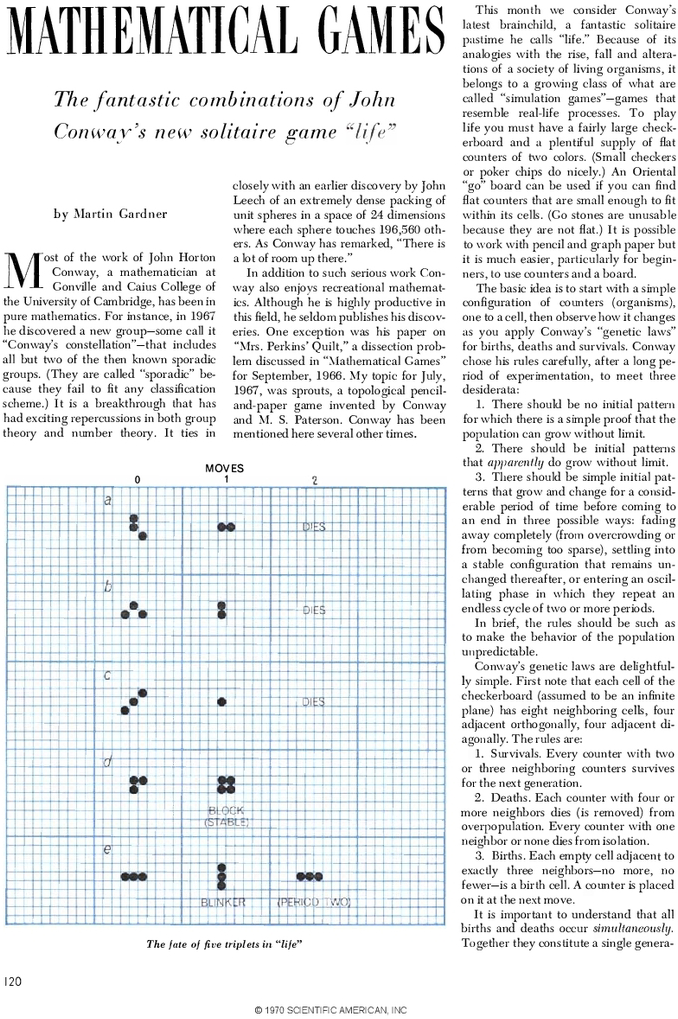
\includegraphics[width=0.75\textwidth]{early_life/sci_am_1970.png}
		\caption{Conway's Game of Life was popularized by the October 1970 issue of \emph{Scientific American}.}\label{fig:sci_am_1970}
	\end{minipage}\hfill
	\begin{minipage}[b]{0.48\textwidth}
		\centering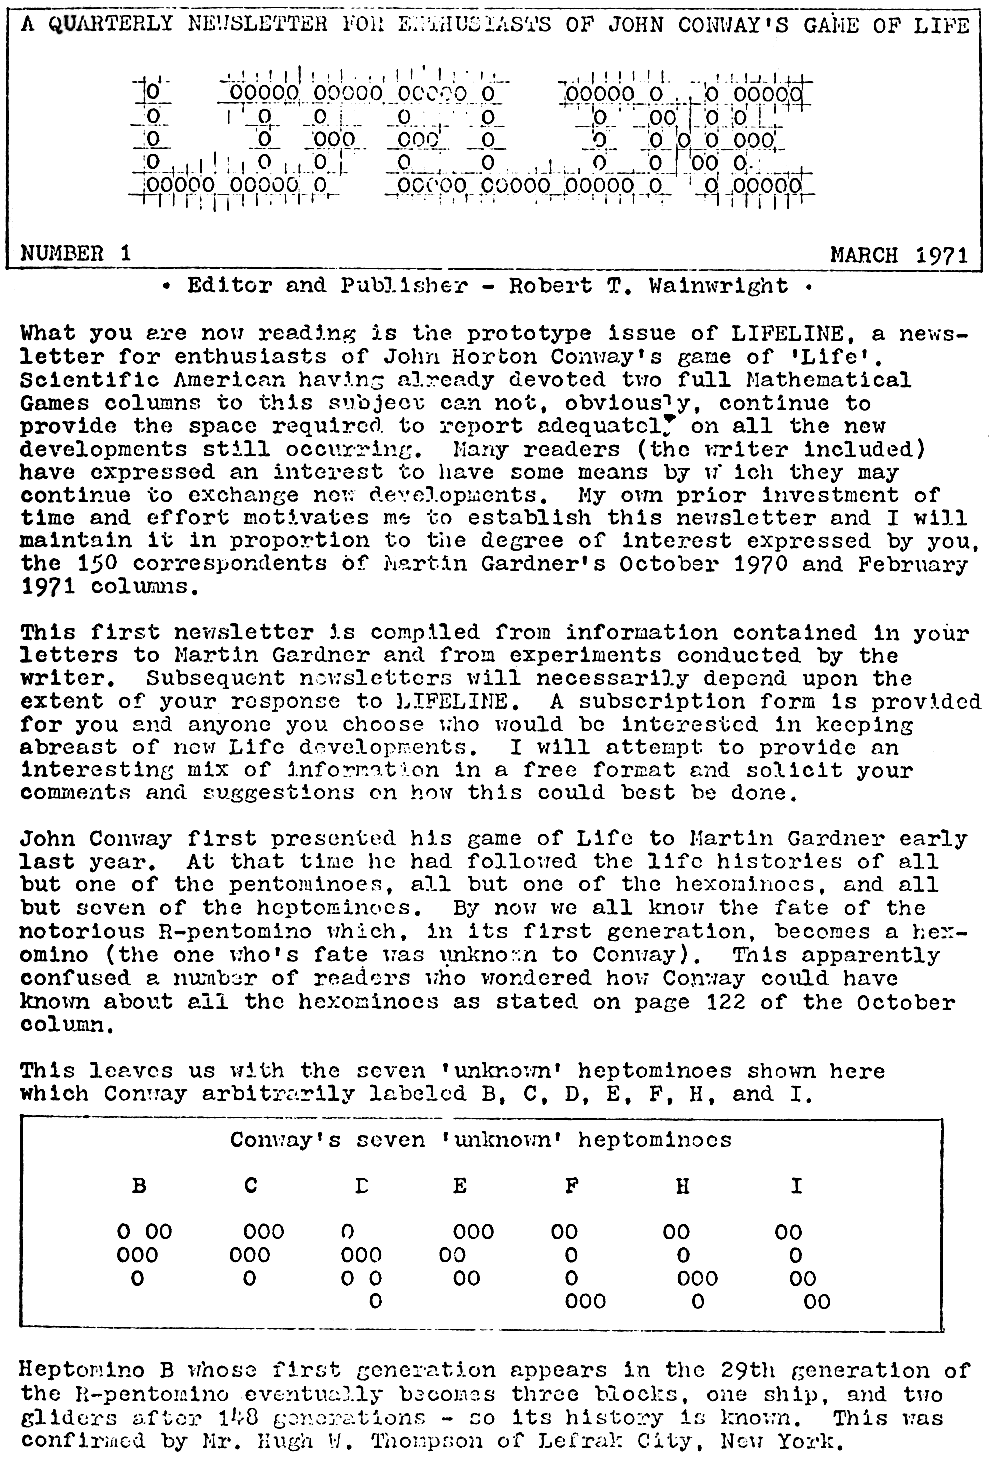
\includegraphics[width=0.75\textwidth]{early_life/lifeline_vol1.png}
		\caption{The front page of the first issue of \emph{Lifeline}, a newsletter for Life enthusiasts that ran from March 1971 to September 1973.}\label{fig:lifeline}
	\end{minipage}
\end{figure}

From 1974 to 2009, Life enthusiasts mostly shared patterns via various private mailing lists, and collections of those patterns made their way to various personal web pages in the 1990s. In 2004, the LifeNews website was launched at \httpurl{pentadecathlon.com}, which posted most interesting new Life discoveries as they were made. Since about 2009, most new discoveries in Life are now reported on the forums at \httpsurl{conwaylife.com}.

Although more advanced techniques are now known for constructing interesting Life objects (indeed, these techniques comprise the majority of the rest of this book), the idea of simply running randomly generated soups to completion to see what remains of them after they stabilize has been a consistent one. However, because computing power was at much more of a premium in 1970 than it is now, and there was no pre-made Life simulation software for early enthusiasts to use, these patterns were often evolved by hand using graph paper, checkers, or the board and stones from the game Go, to represent the Life grid and its live cells.

Furthermore, the methodology that was used back then was somewhat more systematic---instead of generating large random starting configurations, early Lifers investigated the evolution of all possible small starting configurations. These investigations were exactly where the original interest in the T-tetromino,\index{T-tetromino} R-pentomino,\index{R-pentomino} B-heptomino,\index{B-heptomino} stairstep hexomino\index{stairstep hexomino}, and other small polyominoes came from. In fact, the switch engine was originally found by Charles Corderman when he was investigating the evolution of nonominoes (i.e., polyominoes with $9$ live cells), one of which evolves in the exact same way as the switch engine (see Figure~\ref{fig:switch_engine_nonomino}).

Solomon W. Golomb invented the term ``polyomino'' in 1953, and Martin Gardner wrote a popular Mathematical Games article about them a decade before the first article on Conway's Game of Life. Perhaps partly because of this long-standing interest in polyominoes in the mathematical community, the fates of N-cell polyominoes were exhaustively researched very early on, giving rise to the common names of many of the active patterns discussed above.  The Moore-neighborhood equivalent of polyominoes, the N-cell \textbf{polyplets}\index{polyplet}---cell groups that are kingwise-connected rather than rookwise-connected--- are technically just as relevant as a potential source of novelty, but their evolutionary fates were much less thoroughly explored in the early years than the polyominoes.

\begin{figure}[!htb]
	\centering
	\begin{subfigure}{.48\textwidth}
		\centering \embedlink{nonomino}{\vcenteredhbox{\patternimg{0.1}{switch_engine_nonomino_0}} \vcenteredhbox{\genarrow{2}} \vcenteredhbox{\patternimg{0.1}{switch_engine_nonomino_2}}}
		\caption{A nonomino.}\label{fig:switch_engine_nonomino_non}
	\end{subfigure} \ \ \ \ % 
	\begin{subfigure}{.48\textwidth}
		\centering \patternlink{switch_engine}{\vcenteredhbox{\patternimg{0.1}{switch_engine_not_nonomino_0}} \vcenteredhbox{\genarrow{2}} \vcenteredhbox{\patternimg{0.1}{switch_engine_not_nonomino_2}}}
		\caption{A switch engine.}\label{fig:switch_engine_nonomino_not}
	\end{subfigure}
	\caption{The nonomino~(a) evolves in the same way as the switch engine~(b) after $2$ generations.}\label{fig:switch_engine_nonomino}
\end{figure}

Building upon this idea of finding objects by evolving random starting configurations, Achim Flammenkamp ran an automated computer search in 1994 that repeatedly generated random soups and evolved them, keeping a list of all objects that it found in the resulting ash. This search ran until it had accumulated $5 \times 10^9$ (non-distinct) ash objects, which contained a total of $48$ distinct oscillators \cite{Fla94}. He then performed this search again in 2004, this time accumulating $5 \times 10^{10}$ ash objects, and found over $3{\thousep}500$ distinct still lifes and over 80 different oscillators \cite{Fla04}.

Andrzej Okrasinski created a similar program that acted as a screensaver in November~2003. Over the subsequent 5~years, this screensaver catalogued over $4.7 \times 10^{11}$ ash objects, including over $8{\thousep}000$ distinct still lifes and about 180 oscillators, but still the only spaceships that turned up were the four that we have already seen (the glider, LWSS, MWSS, and HWSS) \cite{Okr03}. The screensaver also kept track of how long each starting configuration took to stabilize, and found some new methuselahs in the process, including a 15-cell version of Lidka, which was presented in Table~\ref{tab:small_methuselahs} (it was improved to a 13-cell version by David Bell and then to the more compact 13-cell version presented in that table by Simon Ekström).

In 2009, Nathaniel Johnston created a distributed online search to continue in this vein, called \emph{The Online Life-Like CA Soup Search} (or \emph{TOLLCASS}\index{TOLLCASS} for short). This script had the advantage that multiple people could run it simultaneously on different computers, and their results were automatically uploaded to a central server that organized them. TOLLCASS also worked not just with Conway's Game of Life, but also with a handful of other Life-like cellular automata. The major downside of this script was that it was quite slow, and over the two years that it was active, it catalogued only about one third as many objects as Okrasinski's earlier search.

Finally, Adam P. Goucher launched another distributed online search in 2014 called \emph{apgsearch}\index{apgsearch},\footnote{Officially, the ``apg'' in apgsearch are not its author's initials, but rather stand for \textbf{a}sh \textbf{p}attern \textbf{g}enerator.} which is still active today\footnote{It is available at \httpsurl{catagolue.hatsya.com/apgsearch}.} and is the current state-of-the-art when it comes to soup searching. Like TOLLCASS, it can be used with several different Life-like CA, but with the main advantage of being extremely fast. In the seven years since it began, it has catalogued about $10{\thousep}000$ times as many ash objects as all of the previous searches combined (and this number will likely become out of date very quickly). A summary of these various soup searches that have taken place over the years is provided by Table~\ref{tab:ash_searches}.

\begin{table}[!htb]\vspace*{0.05in}
	\begin{center}		
		\begin{tabular}{l c c l}
			\toprule
			Search Name & Year(s) & Ash Objects Found & Notes \\ \midrule
			Flammenkamp & 1994 & $5.0 \times 10^9$ & first automated soup search \\
			\rowcolor{gray!20} Flammenkamp & 2004 & $5.0 \times 10^{10}$ & -- \\
			Okrasinski & 2003--2008 & $4.7 \times 10^{11}$ & also found methuselahs \\
			\rowcolor{gray!20} TOLLCASS & 2009--2011 & $1.7 \times 10^{11}$ & online search, multiple CA \\
			apgsearch & 2014--present & $1.2 \times 10^{15}$ & online search, multiple CA \\
			\bottomrule
		\end{tabular}
		\caption{A summary of the different soup searches that have taken place over the years.}\label{tab:ash_searches}
	\end{center}
\end{table}


\clearpage% layout fix, remove if layout changes


%%%%%%%%%%%%%%%%%%%%%%%%%%%%%%%%%
\section*{Exercises \hfill \normalfont\textsf{\small solutions to starred exercises on \hyperlink{solutions_early_life}{page \pageref{solutions_early_life}}}}
\label{sec:early_life_exercises}
\addcontentsline{toc}{section}{Exercises}
\vspace*{-0.4cm}\hrulefill\vspace*{-0.3cm}\footnotesize\begin{multicols}{2}\vspace*{-0.4cm}\raggedcolumns\interlinepenalty=10000
	\setlength{\parskip}{0pt}\ifdefined\FORPRINTING\colorlet{ocre}{black}\else%
\fi
	%%%%%%%%%%%%%%%%%%%%%%%%%%%%%%%%%
	
	\begin{problemstar}\label{exer:natural_switch_engine} \probdiff{1}
		Evolve each of the following randomly generated $16 \times 16$ soups and describe the most unusual object that forms.\vspace*{-0.25cm}
		
		\begin{multicols}{2}
			\begin{enumerate}
				\item[\bf\color{ocre}(a)] \raisebox{-\height+\ht\strutbox}{\patternimglink{0.1}{exercise_random_1}}
				
				\item[\bf\color{ocre}(c)] \raisebox{-\height+\ht\strutbox}{\patternimglink{0.1}{exercise_random_3}}
				
				\item[\bf\color{ocre}(b)] \raisebox{-\height+\ht\strutbox}{\patternimglink{0.1}{exercise_random_2}}
				
				\item[\bf\color{ocre}(d)] \raisebox{-\height+\ht\strutbox}{\patternimglink{0.1}{exercise_random_4}}
			\end{enumerate}
		\end{multicols}
	\end{problemstar}
	
	
	\mfilbreak
	
	
	\begin{problem}\label{exer:4_cell_methuselahs}
		What is the longest lifespan of a pattern with:\smallskip
		
		\begin{enumerate}[label=\bf\color{ocre}(\alph*)]
			\item \probdiff{1} $1$ or $2$ live cells?
			% SOLUTION: 1
			
			\item \probdiff{2} $3$ live cells?
			
			\item \probdiff{3} $4$ live cells? [Hint: You could try writing a computer program to help you.]
		\end{enumerate}
	\end{problem}
	
	
	\mfilbreak
	
	
	\begin{problem}\label{exer:pentominoes} \probdiff{1}
		All 12 different pentominoes are displayed below. What are their lifespans?
		
		\begin{center}
			\patternimglink{0.1}{exercise_pentominoes}
		\end{center}
	\end{problem}
	
	
	\mfilbreak
	
	
	\begin{problem}\label{exer:twin_bees_stabilize}
		In this exercise, we will find some alternate stabilizations of the twin bees shuttle from Figure~\ref{fig:twin_bees_shuttle}.\smallskip
		
		\begin{enumerate}[label=\bf\color{ocre}(\alph*)]
			\item \probdiff{1} Try removing some of the blocks from the twin bees shuttle. Which combinations of blocks can you remove while preserving it as a period~46 oscillator?
			% Can remove up to one block from each side
			
			\item \probdiff{2} The still life below is called a \textbf{hat}\index{hat}. Use a hat to stabilize one side of the twin bees shuttle.
			\begin{center}
				\patternimglink{0.1}{hat}
			\end{center}
			% SOLUTION:
			% x = 29, y = 11, rule = B3/S23
			% 17bo$2o15b2o$2o16b2o$13b2o2b2o6bo$25b3o$28bo$25b3o$13b2o2b2o6bo$2o16b2o$2o15b2o$17bo!
		\end{enumerate}
	\end{problem}
	
	
	\mfilbreak
	
	
	\begin{problemstar}\label{exer:find_unstable} \probdiff{2}
		Find a specific generation at which each of the following unstable objects appears in the evolution of the R-pentomino.\smallskip
		
		\begin{enumerate}[label=\bf\color{ocre}(\alph*)]
			\item A T-tetromino.
			
			\item A pre-honey farm.
			
			\item A pi-heptomino.
			
			\item A queen bee.
			
			\item Lumps of muck (in particular, generation~$3$ of the stairstep hexomino).
		\end{enumerate}
	\end{problemstar}
	
	
	\mfilbreak
	
	
	\begin{problem}\label{exer:double_gosper_gun} \probdiff{3}
		Use two blocks and three queen bees to create a ``double'' Gosper glider gun: a gun that emits two streams of gliders.
	\end{problem}
	% SOLUTION:
	% x = 50, y = 13, rule = B3/S23
	%36b2o$38bo$25b2o12bo8b2o$25b2o4bo7bo8b2o$11bo10b2o5b2o8bo$11bobo7b3o5b
	%o2b2o4bo$2o12b2o6b2o6b5ob2o$2o12b2o9b2o4bo$14b2o9b2o$11bobo$11bo11bo
	%15bo$21bobo16bo$22b2o14b3o!
	
	
	\mfilbreak
	
	
	\begin{problemstar}\label{exer:random_symmetric} \probdiff{1}
		Because so many interesting Life objects display some form of symmetry, it is often fruitful to investigate random starting configurations that are also symmetric. Evolve each of the following randomly generated symmetric soups and describe the most unusual object that forms.\smallskip
		
		\begin{enumerate}[label=\bf\color{ocre}(\alph*)]
			\item \raisebox{-\height+\ht\strutbox}{\patternimglink{0.1}{exercise_random_sym_1}}
			
			\item \raisebox{-\height+\ht\strutbox}{\patternimglink{0.1}{exercise_random_sym_2}}
			
			\item \raisebox{-\height+\ht\strutbox}{\patternimglink{0.1}{exercise_random_sym_3}}
			
			\item \raisebox{-\height+\ht\strutbox}{\patternimglink{0.1}{exercise_random_sym_4}}
		\end{enumerate}
	\end{problemstar}
	
	
	\mfilbreak
	
	
	\begin{problemstar}\label{exer:familiar_fours} \probdiff{3}
		There are $5$ formations of $4$ simple objects that commonly occur in ash: the traffic light\index{traffic light}, honey farm\index{honey!farm}, and blockade\index{blockade} that we saw in Section~\ref{sec:evolution}, and the \textbf{fleet}\index{fleet} and \textbf{bakery}\index{bakery} displayed below on the left and right, respectively. These arrangements are collectively called the \textbf{familiar fours}\index{familiar four}.
		
		\begin{center}\captionsetup[subfigure]{labelformat=empty}
			\begin{minipage}{.4\linewidth}
				\centering \patternimglink{0.1}{exercise_fleet}
			\end{minipage} \quad %
			\begin{minipage}{.4\linewidth}
				\centering \patternimglink{0.1}{exercise_bakery}
			\end{minipage}
		\end{center}
		
		\begin{enumerate}[label=\bf\color{ocre}(\alph*)]
			\item Evolve Lidka\index{Lidka} until you see a fleet, and use this evolution to find a $7$-cell predecessor of the fleet.
			
			\item There are at least two different $8$-cell objects that evolve into a bakery. Find one of them. [Hint: Try evolving random soups until you find a bakery, or write a computer program that evolves many different $8$-cell objects.]
		\end{enumerate}
	\end{problemstar}
	
	
	\mfilbreak
	
	
	\begin{problemstar}\label{exer:beehive_pair} \probdiff{2}
		This problem concerns the configuration of two beehives displayed below.
		
		\begin{center}
			\patternimglink{0.1}{beehive_pair}
		\end{center}
		
		\begin{enumerate}[label=\bf\color{ocre}(\alph*)]\vspace*{-0.25cm}
			\item Evolve the pattern until it stabilizes. What happens to the beehives?
			% SOLUTION: They destroy each other.
			
			\item Create a period~30 oscillator that uses this reaction to stabilize two queen bees that are rotated 90 degrees from each other.
			% SOLUTION:
			% x = 25, y = 21, rule = B3/S23
			% 14bo$14bobo$17b2o4b2o$17b2o4b2o$17b2o$14bobo$2b3o9bo2$2bobo$b5o$2o3b2o
			% 13b2o$2o3b2o13b2o3$3bo$b2o2$o2$bo2bo$3b2o!
		\end{enumerate}
	\end{problemstar}
	
	
	\mfilbreak
	
	
	\begin{problemstar}\label{exer:queen_bee_eater_1} \probdiff{2}
		This problem concerns the pattern displayed below. The top-left object is a pre-beehive\index{pre-beehive}, while the bottom-right object is called \textbf{eater~1}\index{eater!1}.
		\begin{center}
			\patternimglink{0.1}{beehive_eater_1}
		\end{center}
		
		\begin{enumerate}[label=\bf\color{ocre}(\alph*)]
			\item Evolve the pattern until it stabilizes. What happens to the pre-beehive and eater~1?
			
			\item Evolve the pre-beehive and eater~1 individually (i.e., not next to each other). Describe what happens to them.
			
			\item Evolve a queen bee until you find a pre-beehive that it leaves behind.
			
			\item Use an eater~1 (instead of a block) to stabilize one side of the queen bee shuttle.
		\end{enumerate}
	\end{problemstar}
	
	
	\mfilbreak
	
	
	\begin{problem}\label{exer:bunnies} \probdiff{1}
		The $9$-cell methuselah displayed below is called \textbf{bunnies}\index{bunnies}.\footnote{Its $1$-generation successor, which is called \textbf{rabbits}\index{rabbits}, was found by Andrew Trevorrow in 1986. This version was subsequently found independently by Robert Wainwright and Andrew Trevorrow.}
		
		\begin{center}
			\patternimglink{0.1}{exercise_bunnies}
		\end{center}
		
		\begin{enumerate}[label=\bf\color{ocre}(\alph*)]
			\item What is its lifespan?
			
			\item It eventually evolves in the same way as each of bunnies~9 and bunnies~10b from Table~\ref{tab:small_methuselahs}. Find the first generation of each object's evolution where they match.
		\end{enumerate}
	\end{problem}
	
	
	\mfilbreak
	
	
	\begin{problem}\label{exer:edna}\index{Edna} \probdiff{1}
		The methuselah displayed below is named \textbf{Edna}.\footnote{Found by Erik de Neve in January 2010.}
		
		\begin{center}
			\patternimglink{0.08}{edna}
		\end{center}
		
		\begin{enumerate}[label=\bf\color{ocre}(\alph*)]
			\item What is its lifespan?
			% SOLUTION: 31192
			
			\item What objects can be found in its ash after this pattern stabilizes? Are there any objects that we did not give names to in this chapter?
		\end{enumerate}
	\end{problem}


	\mfilbreak
	
	
	\begin{problem}\label{exer:8cell_methuselah} \probdiff{1}
		An $8$-cell methuselah with a longer lifespan than the $8$-cell methuselah from Table~\ref{tab:small_methuselahs} (but with a significantly larger bounding box) is displayed below.\footnote{Found by Nick Gotts in 2019.} What is its lifespan?
		
		\begin{center}
			\patternimglink{0.1}{exercise_8cell_meth}
		\end{center}
	\end{problem}
	% 14321
	
	
	\mfilbreak
	
	
	\begin{problem}\label{exer:noahs_ark} \probdiff{2}
		An ark called \textbf{Noah's ark}\index{Noah's ark} is displayed below.\footnote{This ark was found in 1971 by Charles Corderman, and was the first-discovered ark. Its name refers to the fact that the debris it leaves behind contains pairs of many different objects. The general term ``ark'' is derived from the name of this pattern.} What is the period of this pattern, and what objects does it leave behind as it moves?
		
		\begin{center}
			\patternimglink{0.1}{exercise_noahs_ark}
		\end{center}
	\end{problem}

	
	\mfilbreak
	
	
	\begin{problem}\label{exer:goe_height_1_exercise} \probdiff{2}
		Find a parent of the following $1$-cell-thick pattern: \\[0.04em]
		
		\begin{center}
			\vspace*{-1em}\patternimglink{0.09}{goe_height_1_exercise}
		\end{center}
	\end{problem}
	
	
	\clearpage
	
	
	\begin{problemstar}\label{exer:goe_theorem} \probdiff{4}
		In the proof of Theorem~\ref{thm:garden_of_eden_exists}, we claimed that the inequality $(2^{36}-1)^{n^2} < 2^{(6n-2)^2}$ holds whenever $n$ is large enough.\smallskip
		
		\begin{enumerate}[label=\bf\color{ocre}(\alph*)]
			\item Find a formula for the smallest value of $n$ for which this inequality holds, and then use computer software to compute its exact value.
			% ceil(2/(6-sqrt(log_2(2^36-1)))) = 1143185077171
			
			\item We can get slightly smaller values of $n$ that lead to Gardens of Eden by considering more tiles that evolve in the same way. Instead of just using the two $6 \times 6$ tiles that we presented in the proof of Theorem~\ref{thm:garden_of_eden_exists}, we could have used the set of \emph{five} tiles displayed below without changing the method of proof significantly. What is the relevant inequality that we need to check? What is the smallest value of $n$ for which this new inequality holds?
			
			\begin{center}
				\patternimg{0.087}{goe_theorem_tiles_more}\\[1em]
			\end{center}
			
			\item Alternatively, we can get smaller values of $n$ leading to Gardens of Eden by using $5 \times 5$ tiles. If we re-do the proof of Theorem~\ref{thm:garden_of_eden_exists} using the $5 \times 5$ tiles displayed below, what is the relevant inequality that we need to check? What is the smallest value of $n$ for which this new inequality holds?
			
			\begin{center}
				\patternimg{0.08}{goe_theorem_tiles_5x5}
			\end{center}
			
			\item Why can't we replace the $6 \times 6$ or $5 \times 5$ tiles with the $4 \times 4$ tiles displayed below? What part of the proof breaks down?
			
			\begin{center}
				\patternimg{0.08}{goe_theorem_tiles_4x4}
			\end{center}
		\end{enumerate}
	\end{problemstar}
	
	
	\vspace*{4cm}
	
	
	\begin{problemstar}\label{exer:ark} \probdiff{2}
		The 19-cell pattern displayed below consists of two switch engine predecessors and a blinker,\footnote{This pattern was found by Nick Gotts in February 2005.} and takes a staggering $6{\thousep}526{\thousep}589$ generations to stabilize.
		
		\begin{center}
			\patternimglink{0.1}{exercise_ark}
		\end{center}
		
		\begin{enumerate}[label=\bf\color{ocre}(\alph*)]
			\item Evolve the pattern to see how it behaves. What effect does the blinker have that makes it live so much longer than the ark in Figure~\ref{fig:ark_736692}?
			
			\item What causes this ark to stabilize?
			
			\noindent [Hint: Compare the evolution of this ark with the evolution presented in Figure~\ref{fig:ark_736692_stabilized}, which shows the stabilization happening as a result of a path being cleared for the backward-flying gliders.]
		\end{enumerate}
	\end{problemstar}
	
	
	\mfilbreak
	
	
	\begin{problem}\label{exer:goe_theorem_limit} \probdiff{3}
		In the proof of Theorem~\ref{thm:garden_of_eden_exists}, we claimed that the inequality $(2^{36}-1)^{n^2} < 2^{(6n-2)^2}$ holds whenever $n$ is large enough. Prove the stronger statement that
		\[
		\lim_{n\rightarrow\infty}\frac{(2^{36}-1)^{n^2}}{2^{(6n-2)^2}} = 0,
		\]
		and hence the vast majority of large patterns are Gardens of Eden. [Hint: Use the fact that $a^b = 2^{b\log_2(a)}$.]
	\end{problem}
	
	
	\mfilbreak
	
	
	\begin{problem}\label{exer:goe_jls}
		A computer program called \emph{JavaLifeSearch}\index{JavaLifeSearch}\footnote{Created by Karel Suhajda, based on earlier programs by David Bell, Dean Hickerson, and Jason Summers.} can be used to find predecessors of Life patterns (or show that none exist). Usage instructions and download links can be found at \httpsurl{conwaylife.com/wiki/JavaLifeSearch}.\smallskip
		
		\begin{enumerate}[label=\bf\color{ocre}(\alph*)]
			\item \probdiff{3} Use JavaLifeSearch to find a predecessor of the following pattern:
			
			\begin{center}
				\patternimg{0.1}{exercise_goe_jls}
			\end{center}
			
			\item \probdiff{4} Use JavaLifeSearch to verify that the patterns from Figure~\ref{fig:goe_records} really are orphans.
			
			\item \probdiff{5} Use JavaLifeSearch to verify that the pattern from Figure~\ref{fig:grandparentless} really does not have any grandparents.
		\end{enumerate}
	\end{problem}
	
	%% EXERCISE END COMMANDS
\end{multicols}
\normalsize\vspace*{0.01cm}\ifdefined\FORPRINTING\colorlet{ocre}{rawocre}\else%
\fi
%% DONE EXERCISE END COMMANDS
